\documentclass{beamer}%[aspectratio=169,10pt]{beamer}

\usetheme[progressbar=frametitle]{metropolis}
\usepackage{appendixnumberbeamer}

\usepackage{tikz}

\usepackage{booktabs}
\usepackage[scale=2]{ccicons}

\usepackage{pgfplots}
\usepgfplotslibrary{dateplot}

\usepackage{xspace}
\newcommand{\themename}{\textbf{\textsc{metropolis}}\xspace}

\usepackage{xcolor}
\definecolor{aliceblue}{rgb}{0.94, 0.97, 1.0}
\definecolor{alizarin}{rgb}{0.82, 0.1, 0.26}
\definecolor{blue-green}{rgb}{0.0, 0.87, 0.87}
% \setbeamercolor{normal text}{ fg=alizarin , bg=aliceblue}
\setbeamercolor{alerted text}{ fg=alizarin , bg=aliceblue}
\setbeamercolor{example text}{ fg=blue-green , bg=aliceblue}

\setbeamercolor{block title alerted}{fg=alizarin , bg=white}
\setbeamercolor{block body alerted}{fg=black , bg=white}

\addtobeamertemplate{block color}{%
  \Salmon}{}
\setbeamercolor{postit}{bg=white!30!white}


% \usepackage[spanish]{babel}
\usepackage[utf8]{inputenc}
%\usepackage[spanish]{babel}
%\addto\shorthandsspanish{\spanishdeactivate{~<>}}

\usepackage{tikz}

\usepackage[sfdefault]{FiraSans} %% option 'sfdefault' activates Fira Sans as the default text font
\usepackage[T1]{fontenc}
\renewcommand*\oldstylenums[1]{{\firaoldstyle #1}}

\setlength{\parskip}{0.2em}
%\setlength{\intextsep}{0pt plus 2pt}

\setbeamerfont{caption}{size=\tiny}
\setlength\abovecaptionskip{-3pt}

\title{Spatiotemporal characteristics of solar resource and photovoltaic productivity over the Euro-Mediterranean area}
\subtitle{A climate perspective}
%\date{\today} 
\date{24th may 2019}
\author{Claudia Guti\'errez}
%\institute{Instituto de Ciencias Ambientales-UCLM}
\institute[ICAM] % (optional, but mostly needed)
 {
   \inst{1}
   Facultad de Ciencias Ambientales y Bioqu\'imica\\
   Universidad de Castilla-La Mancha, Toledo, Spain
}

%  % - Use the \inst command only if there are several affiliations.
%  % - Keep it simple, no one is interested in your street address.

\titlegraphic{
  \tikz[overlay,remember picture]
  \node[at=(current page.south east), anchor=south east] {
    
\includegraphics[height=1cm]{uclm.png}%[height=1cm]
  };
}

      
\begin{document}

\maketitle

\begin{frame}[plain]{Index}                                                                                              \tableofcontents                                                                                                       %You might wish to add the option [pausesections]
\end{frame}

\section{Context and introduction}

\subsection{Energy transition}

\begin{frame}[fragile]{Energy transition}
\begin{figure}
\centering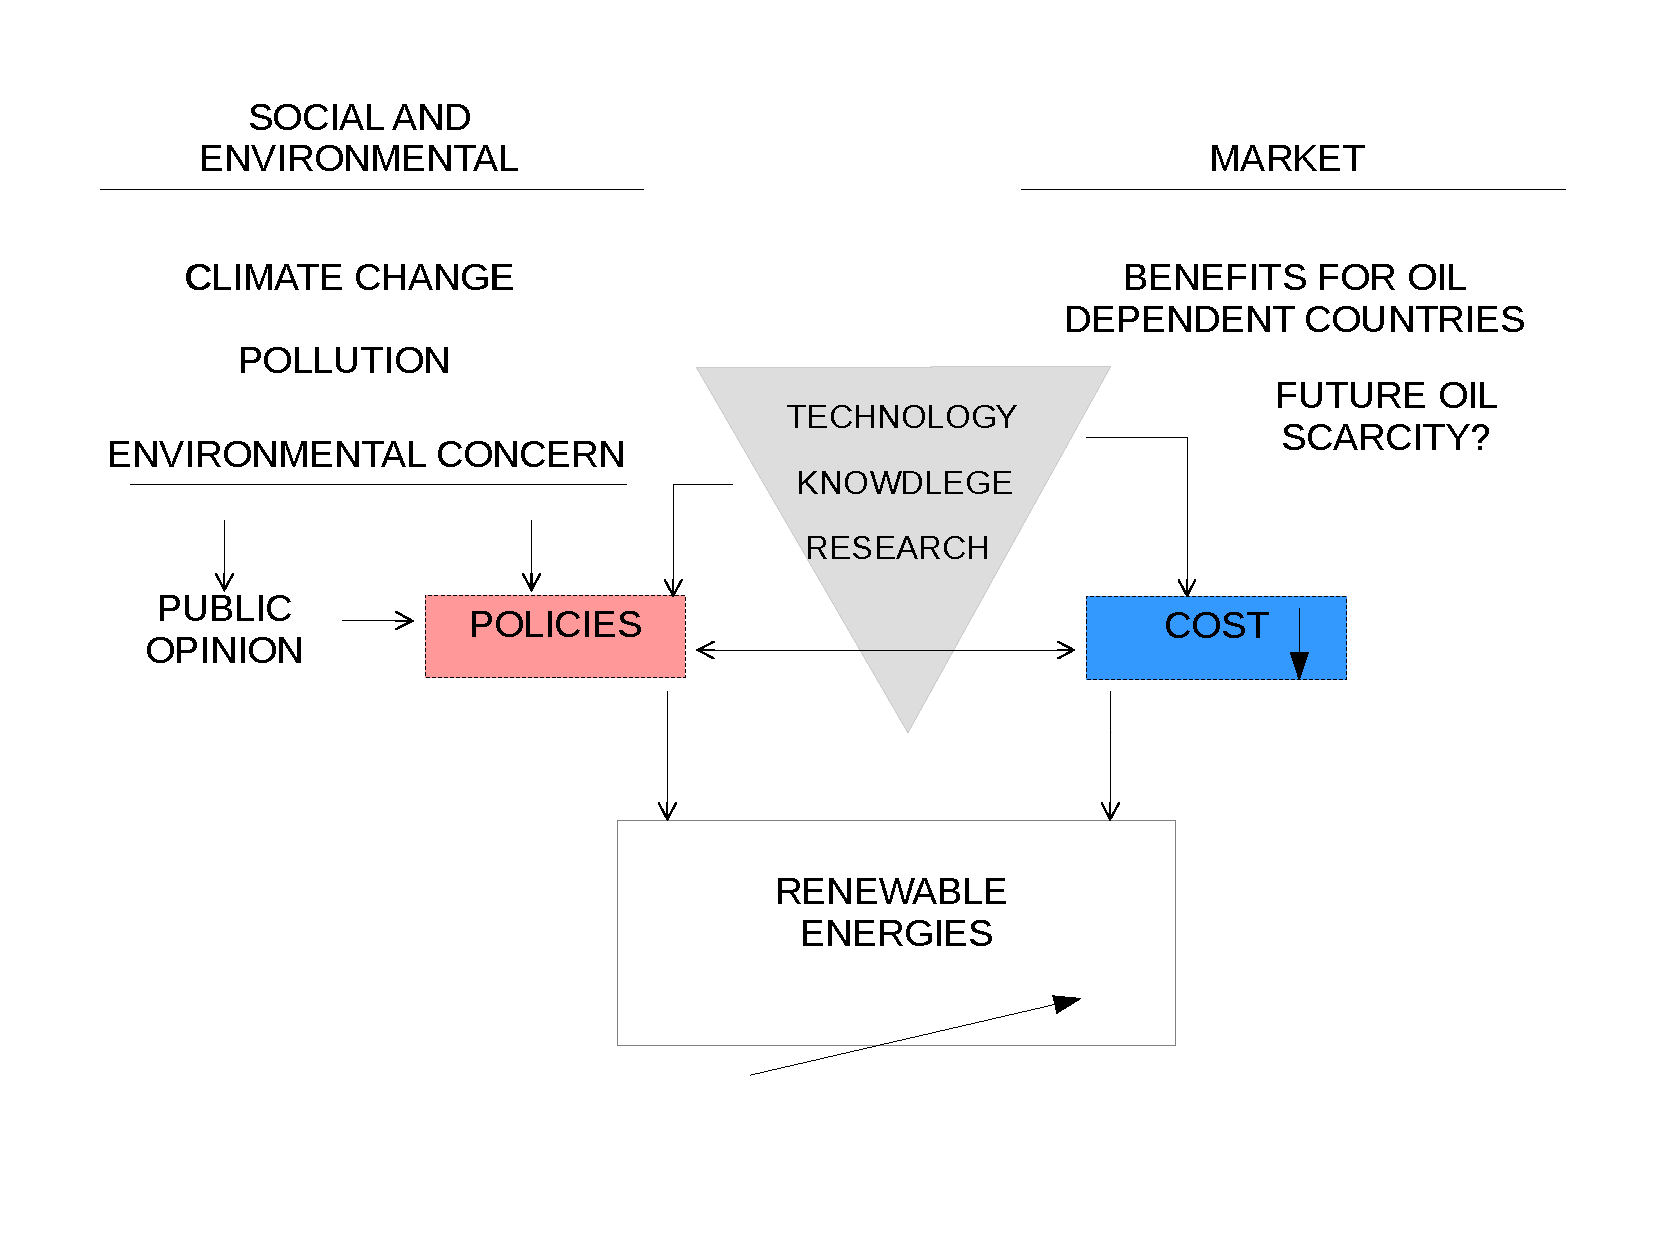
\includegraphics[scale=0.4]{contexto.pdf}
\end{figure}
\end{frame}

\begin{frame}[fragile]{Energy transition}
\begin{figure}
\centering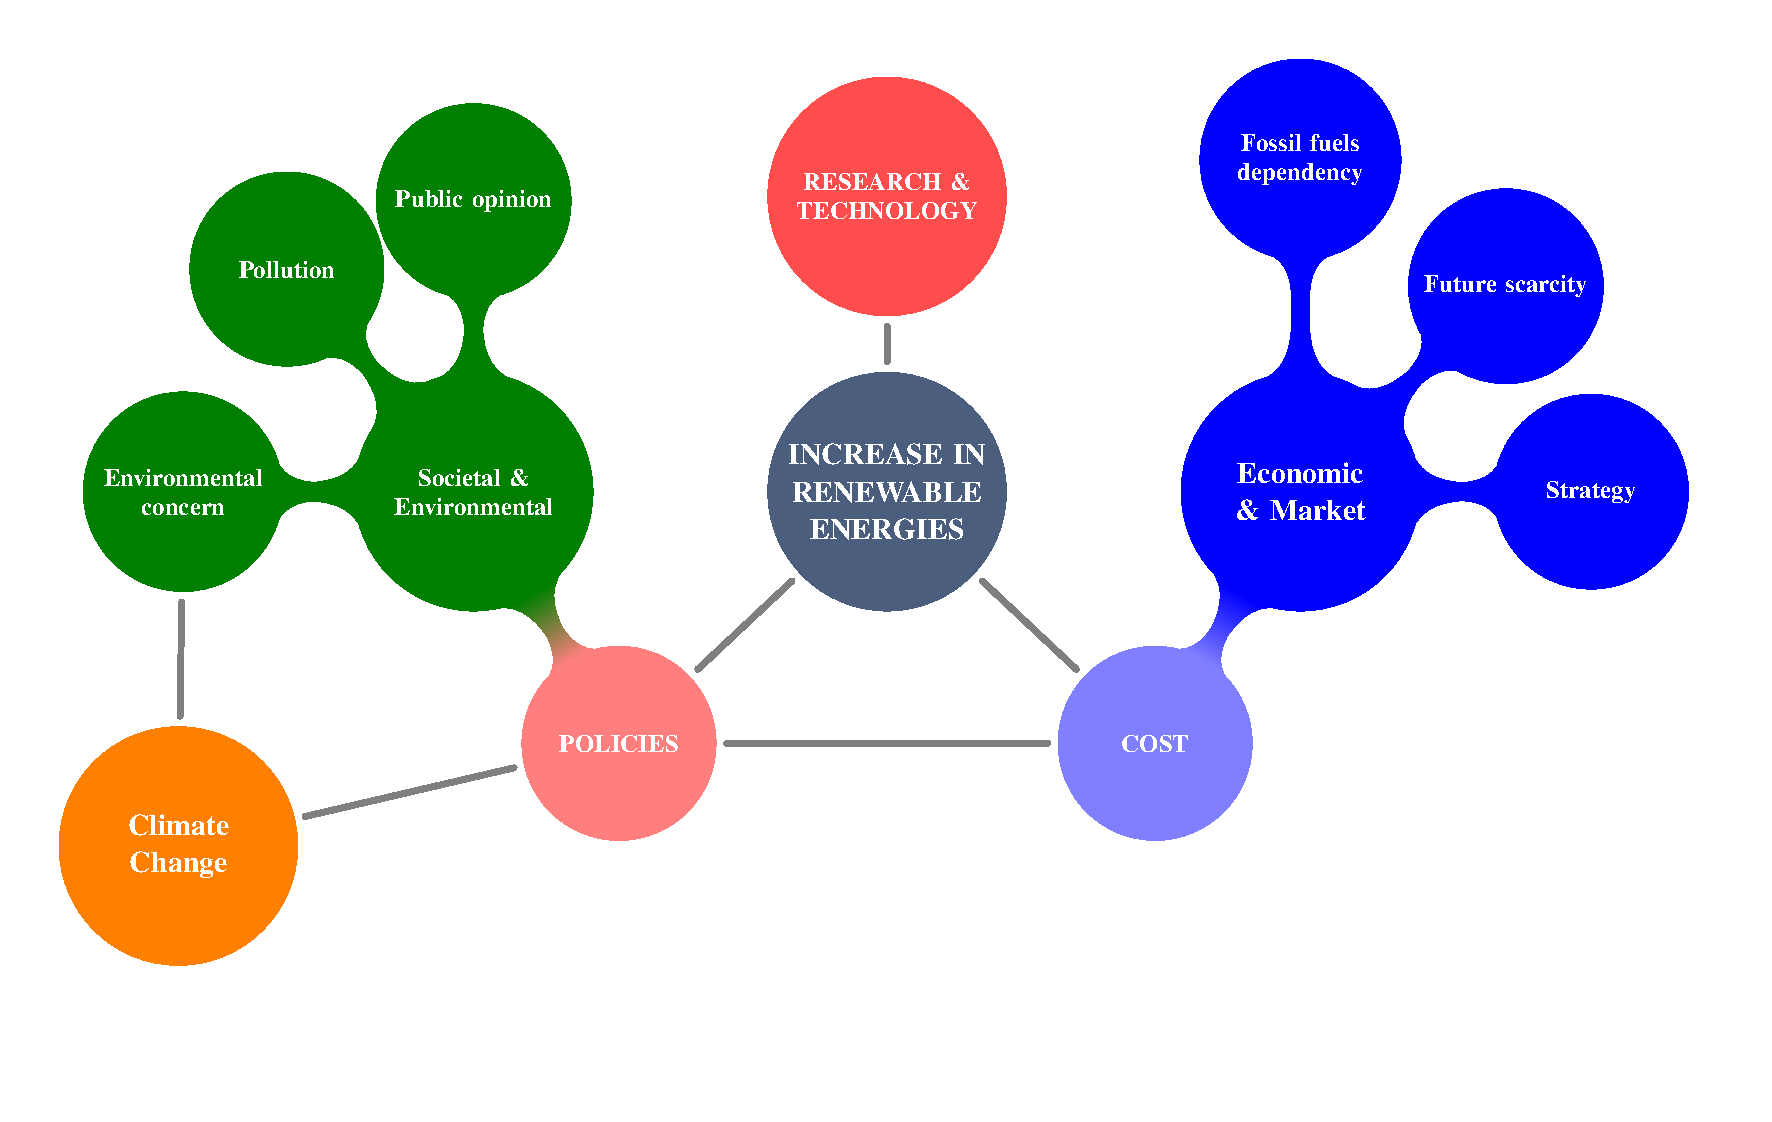
\includegraphics[scale=0.42]{diagram.pdf}
\end{figure} 
\end{frame}

% \begin{frame}[fragile]{Energy transition}
% \begin{figure}
% \centering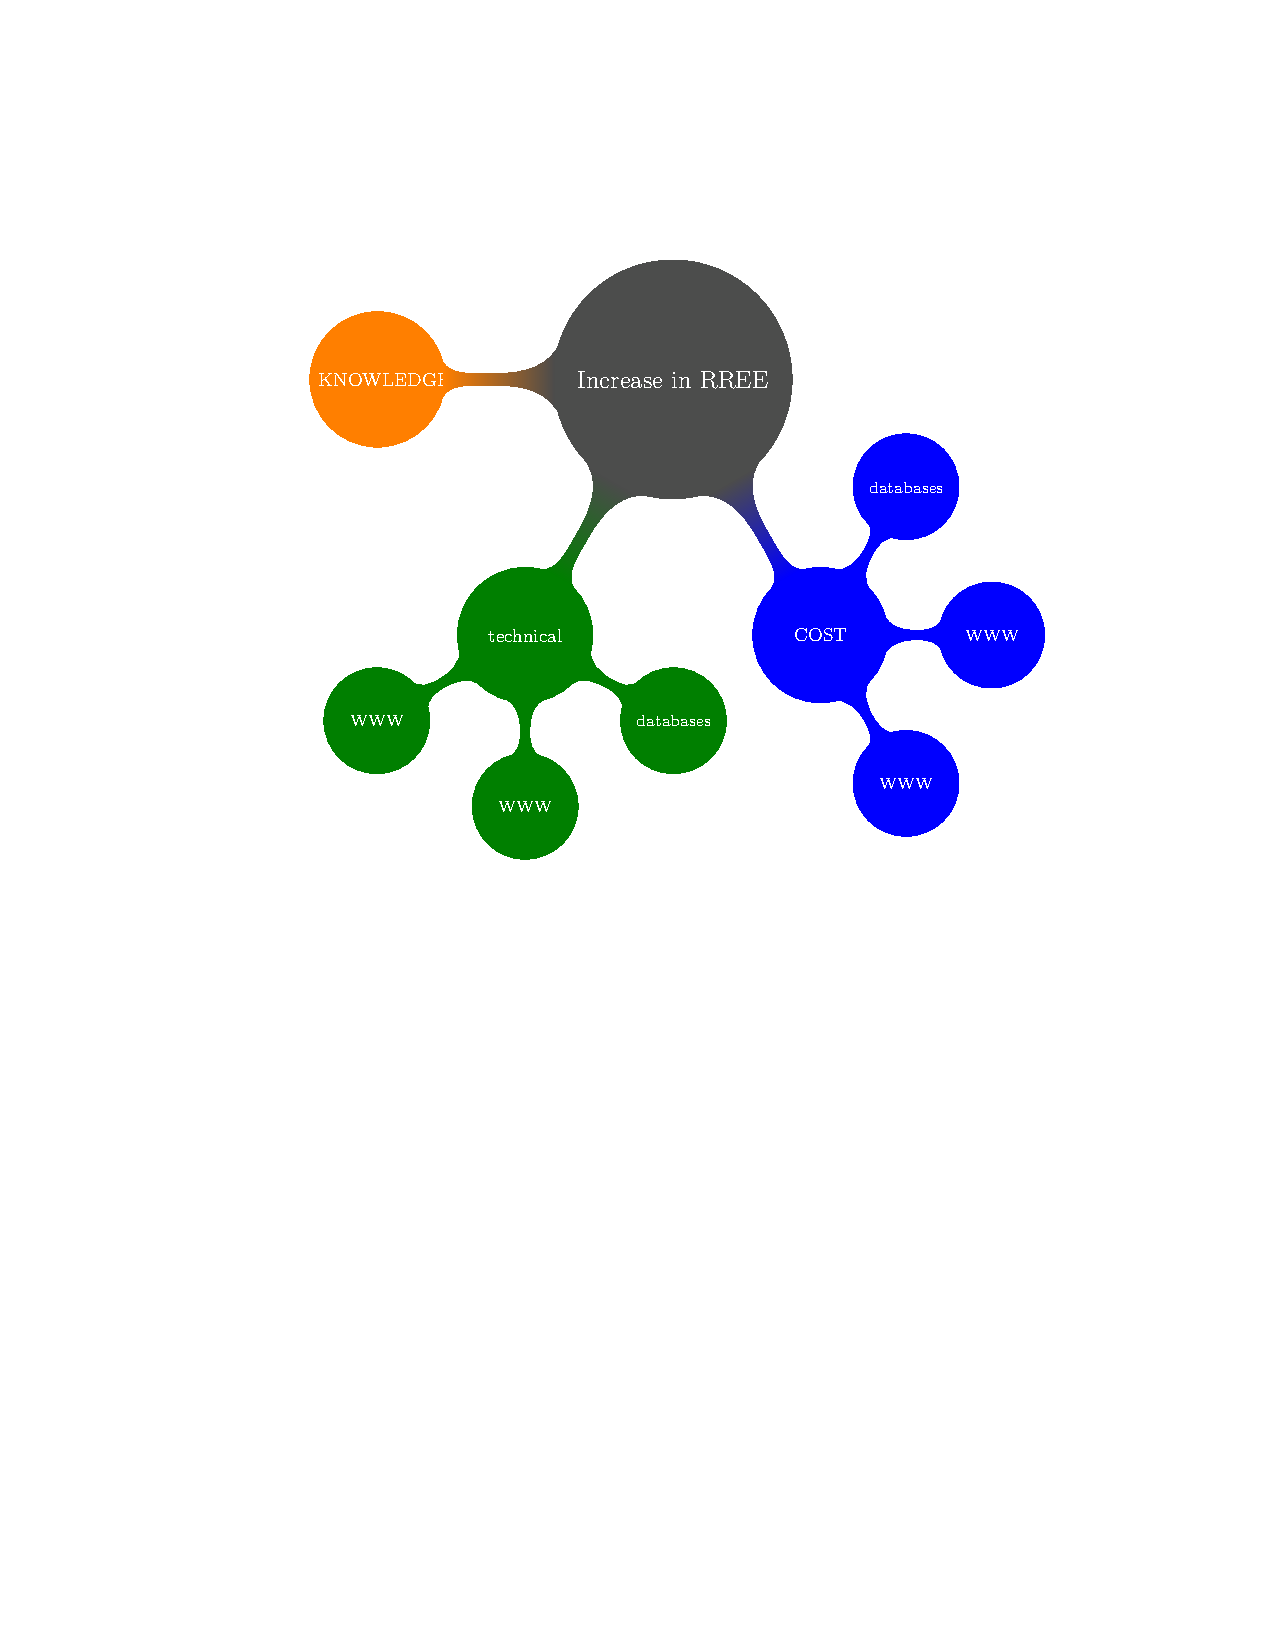
\includegraphics[scale=0.42]{diagram2.pdf}
% \end{figure} 
% \end{frame}

% \begin{frame}[fragile]{Energy transition}
% \begin{figure}
% \centering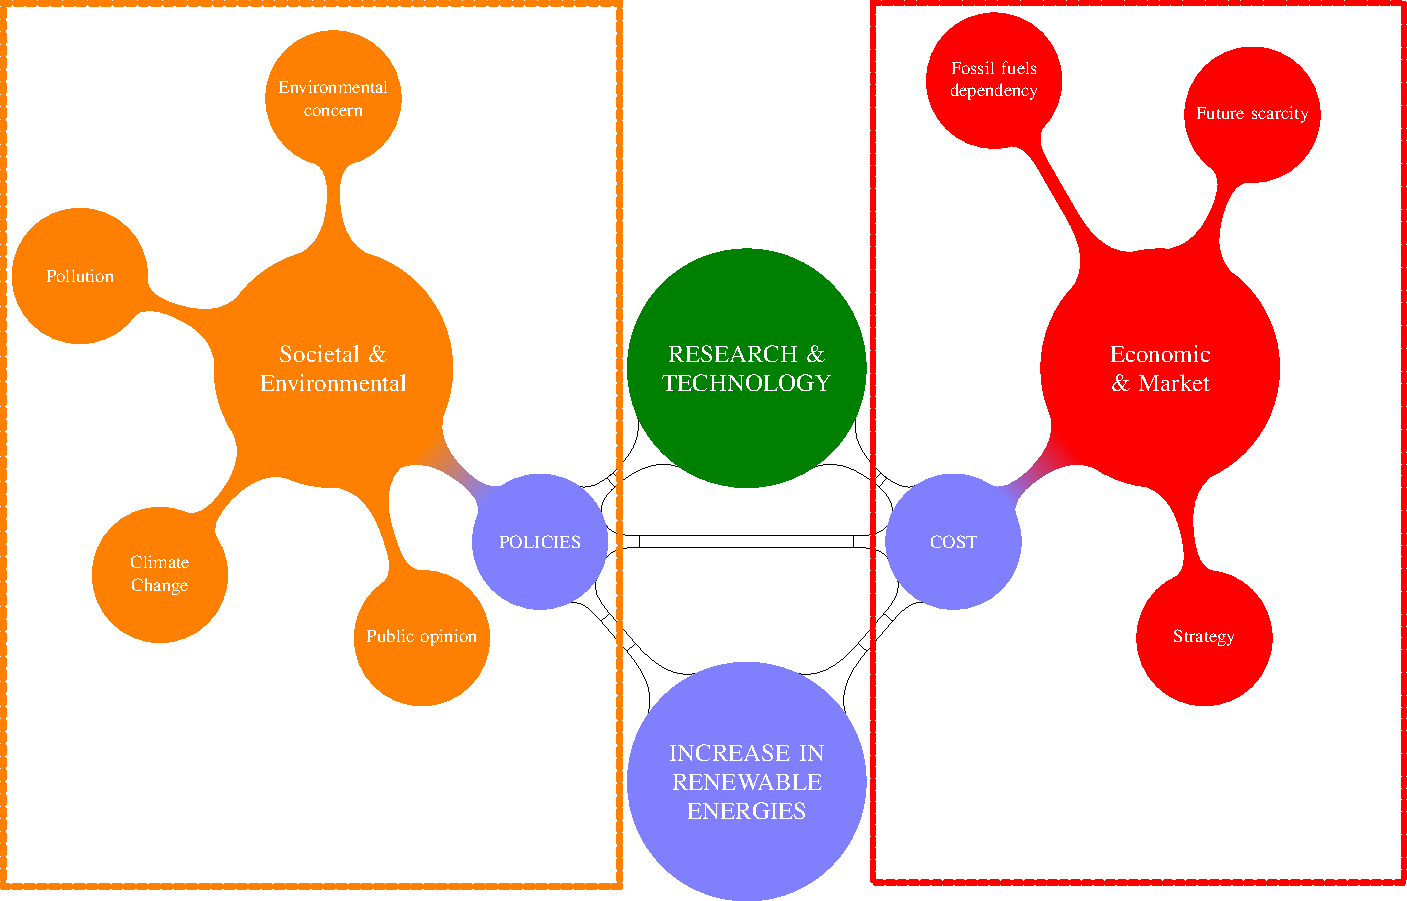
\includegraphics[scale=0.42]{diagram3.pdf}
% \end{figure} 
% \end{frame}

\begin{frame}[fragile]{Energy transition}
\begin{figure}
\centering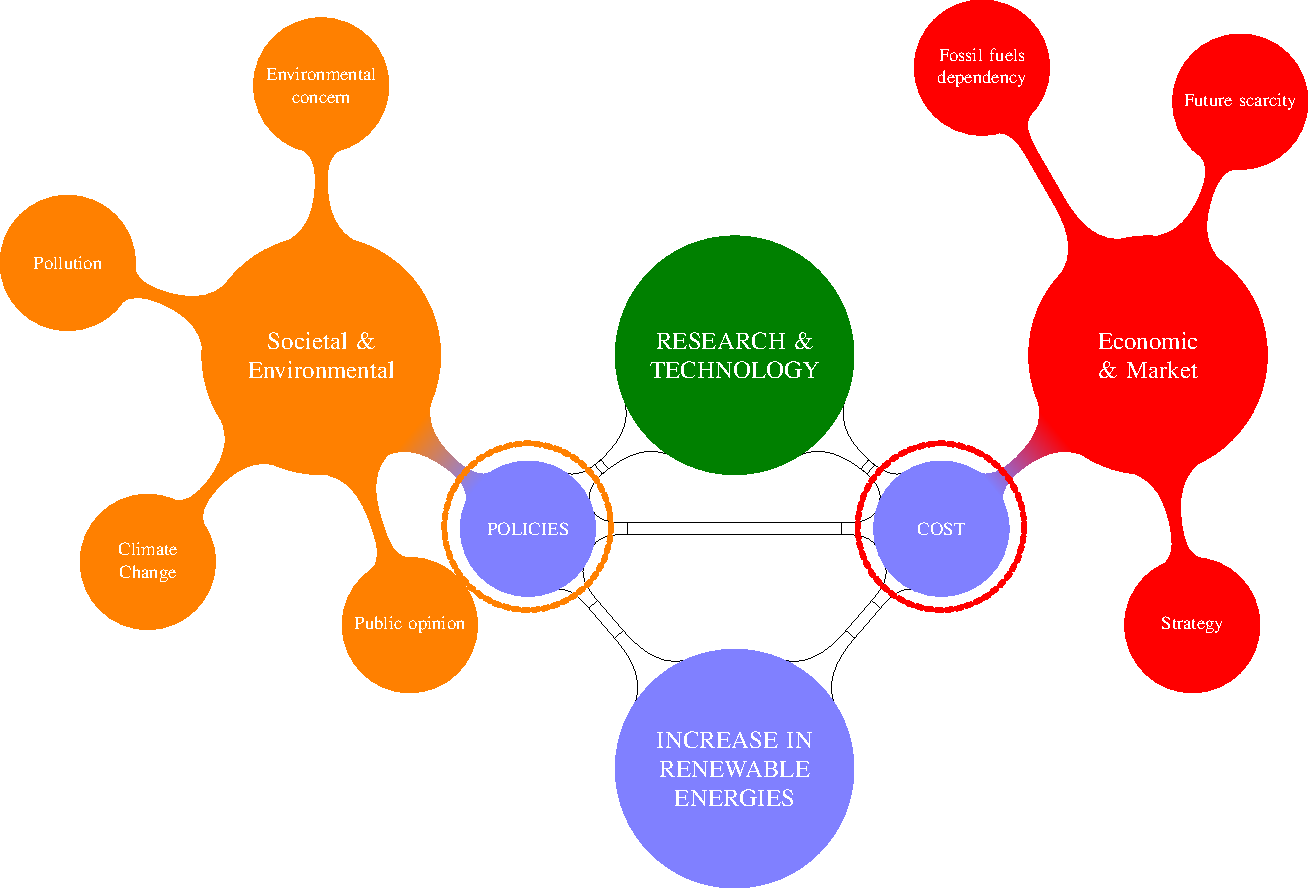
\includegraphics[scale=0.42]{diagram4.pdf}
\end{figure} 
\end{frame}

\begin{frame}[fragile]{Energy transition}
\begin{figure}
\centering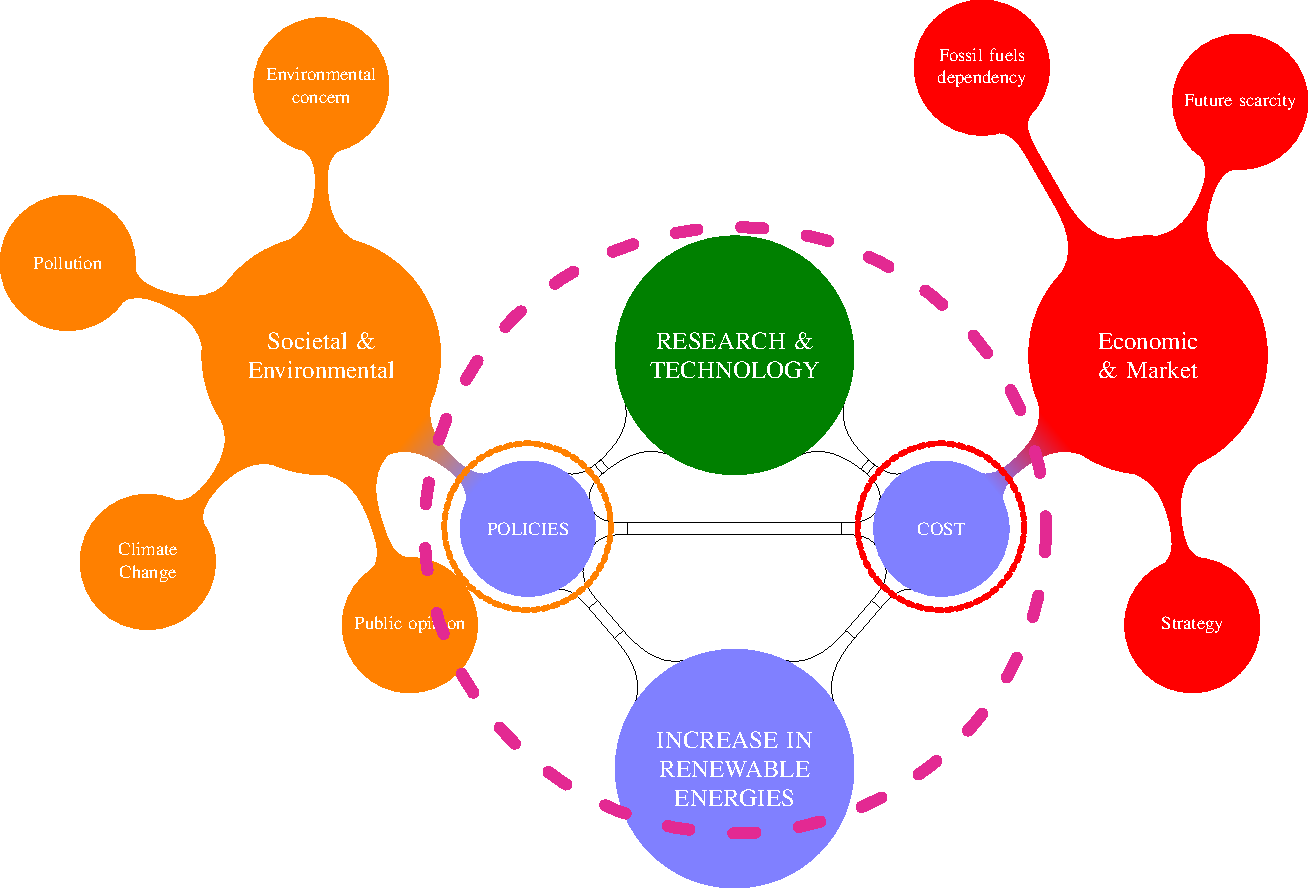
\includegraphics[scale=0.42]{diagram5pdf.pdf}
\end{figure} 
\end{frame}


\begin{frame}[fragile]{Photovoltaic}
\begin{itemize}
\item Increase in \textbf{\alert{photovoltaic (PV) capacity}}
\item Continous growth in projected \textbf{\alert{trends}}.
\item Global increase leaded by China  
\end{itemize}
\begin{figure}
\centering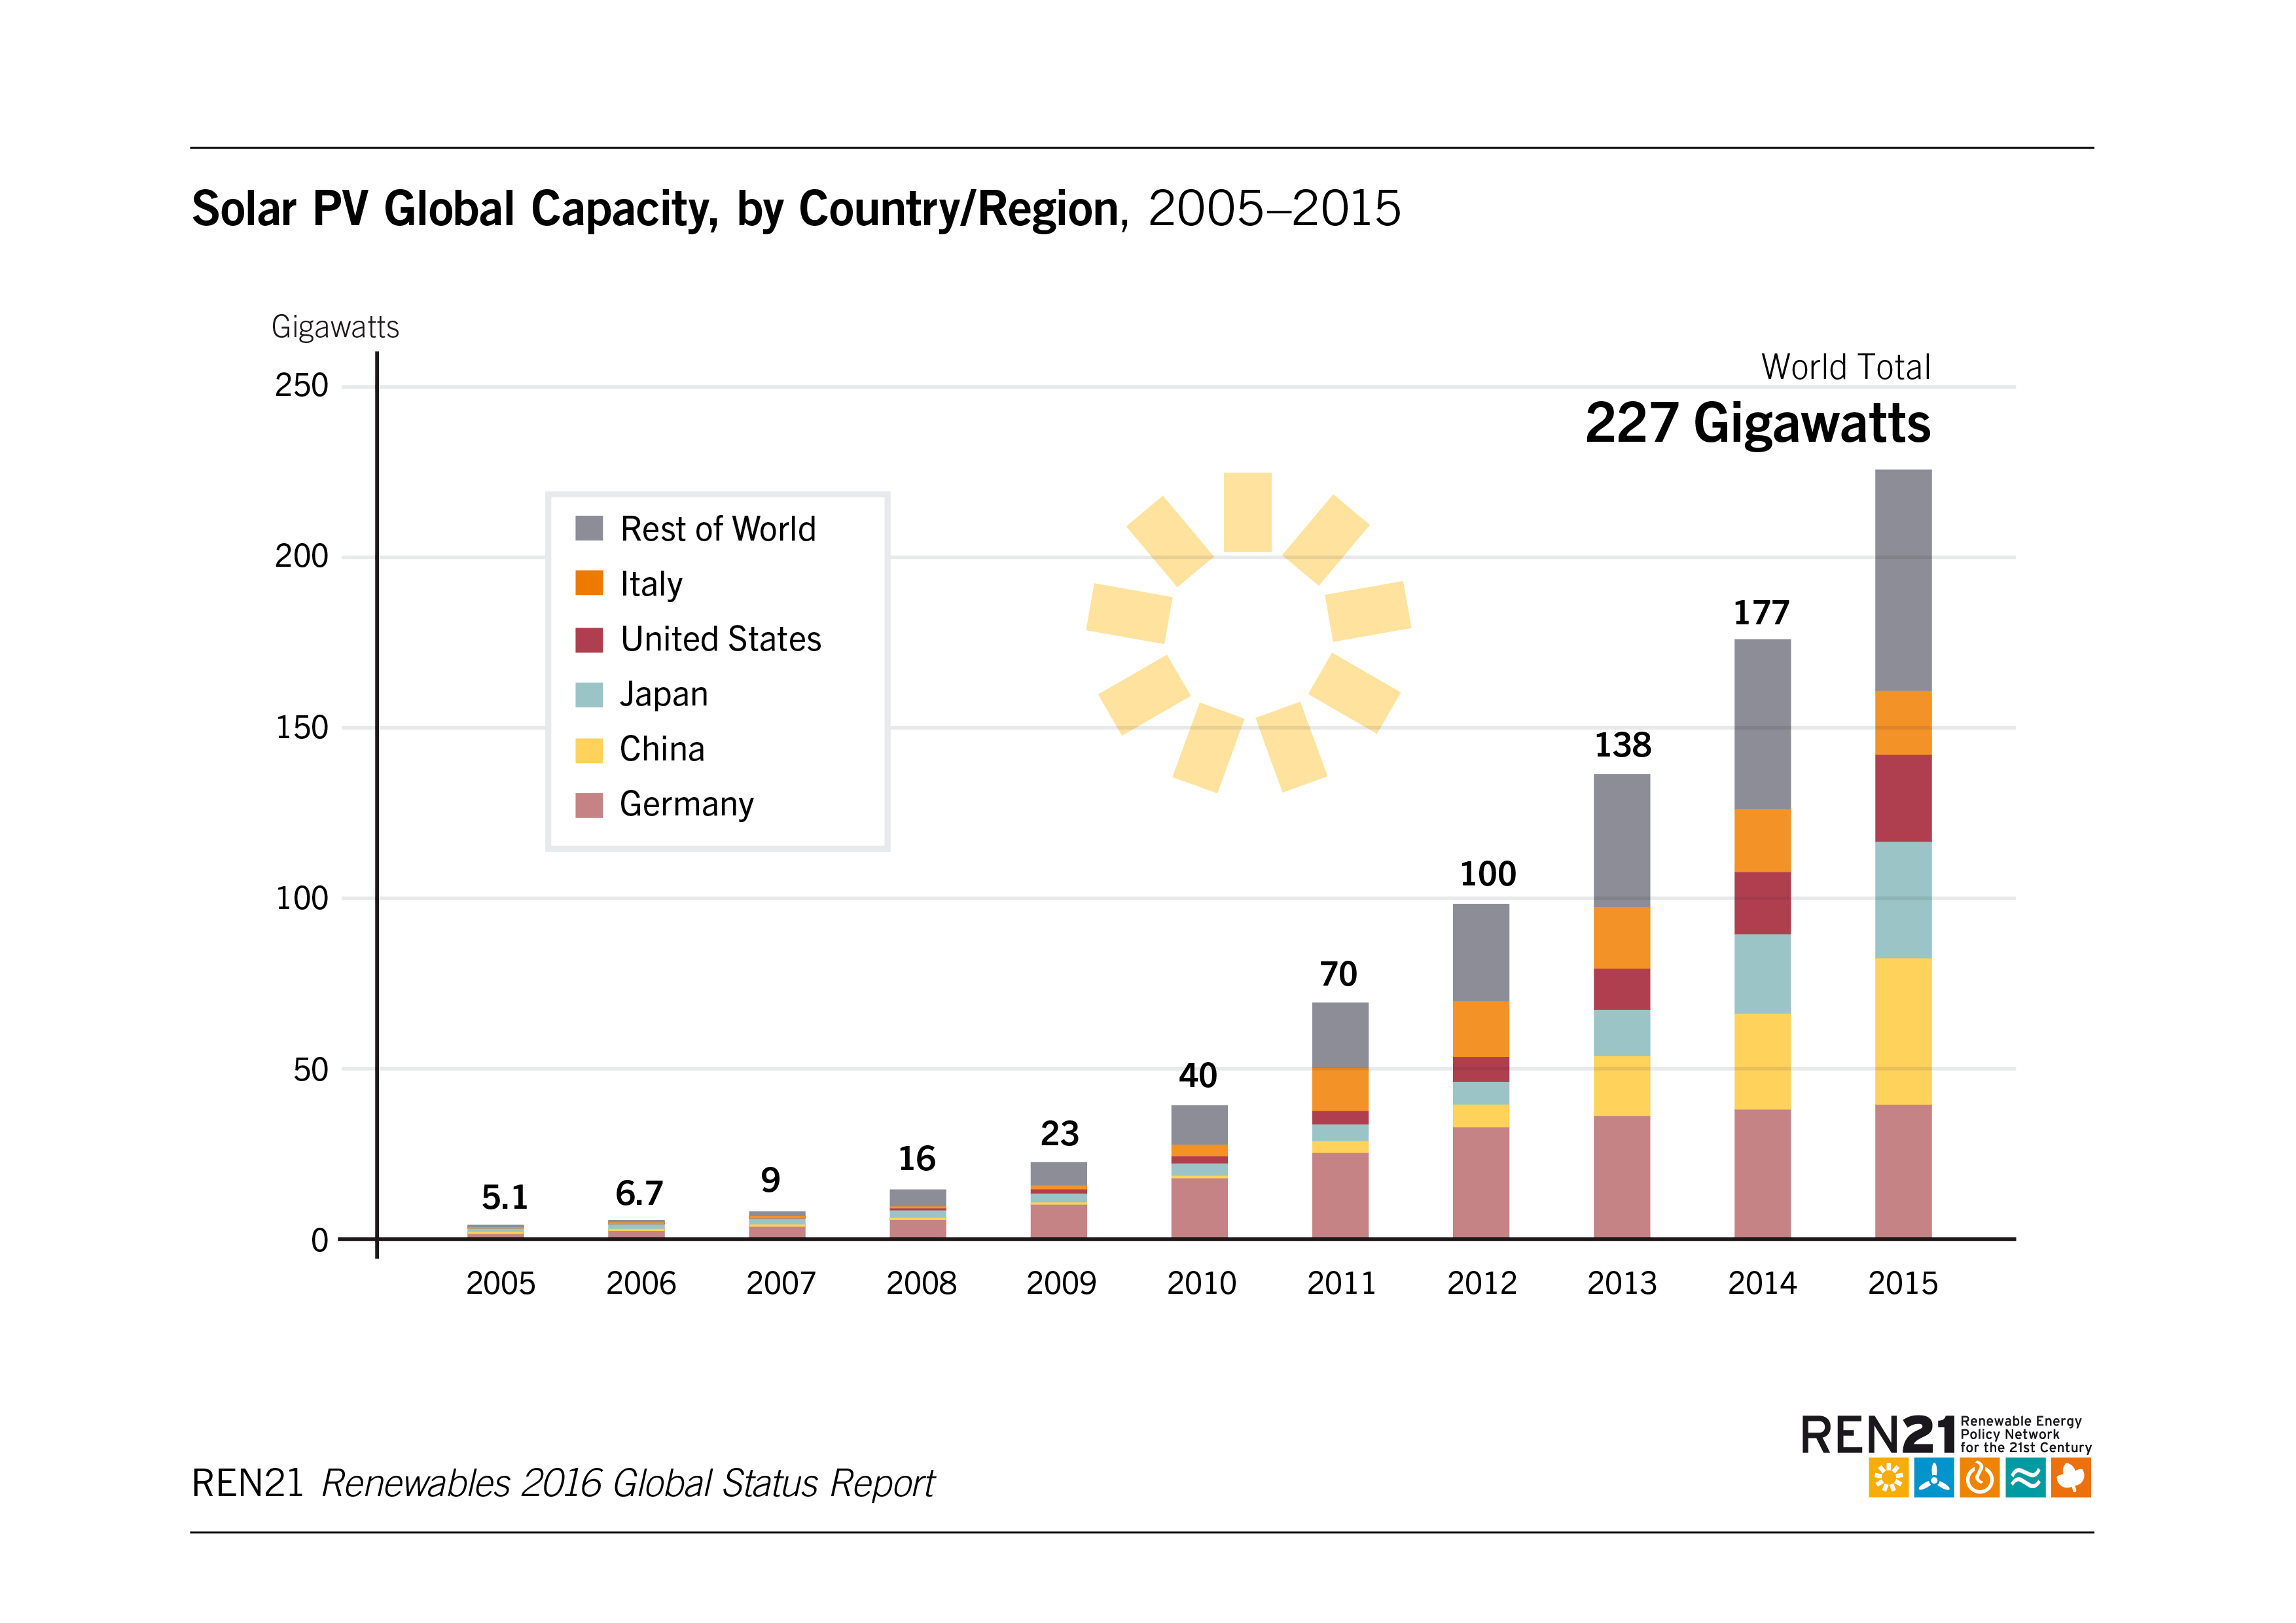
\includegraphics[scale=0.3]{GSR_2016_Figure_15}
\end{figure}
\end{frame}


\subsection{VRE}
 
% {
% \usebackgroundtemplate{\tikz\node[opacity=1, inner sep=0pt, outer sep=0pt]{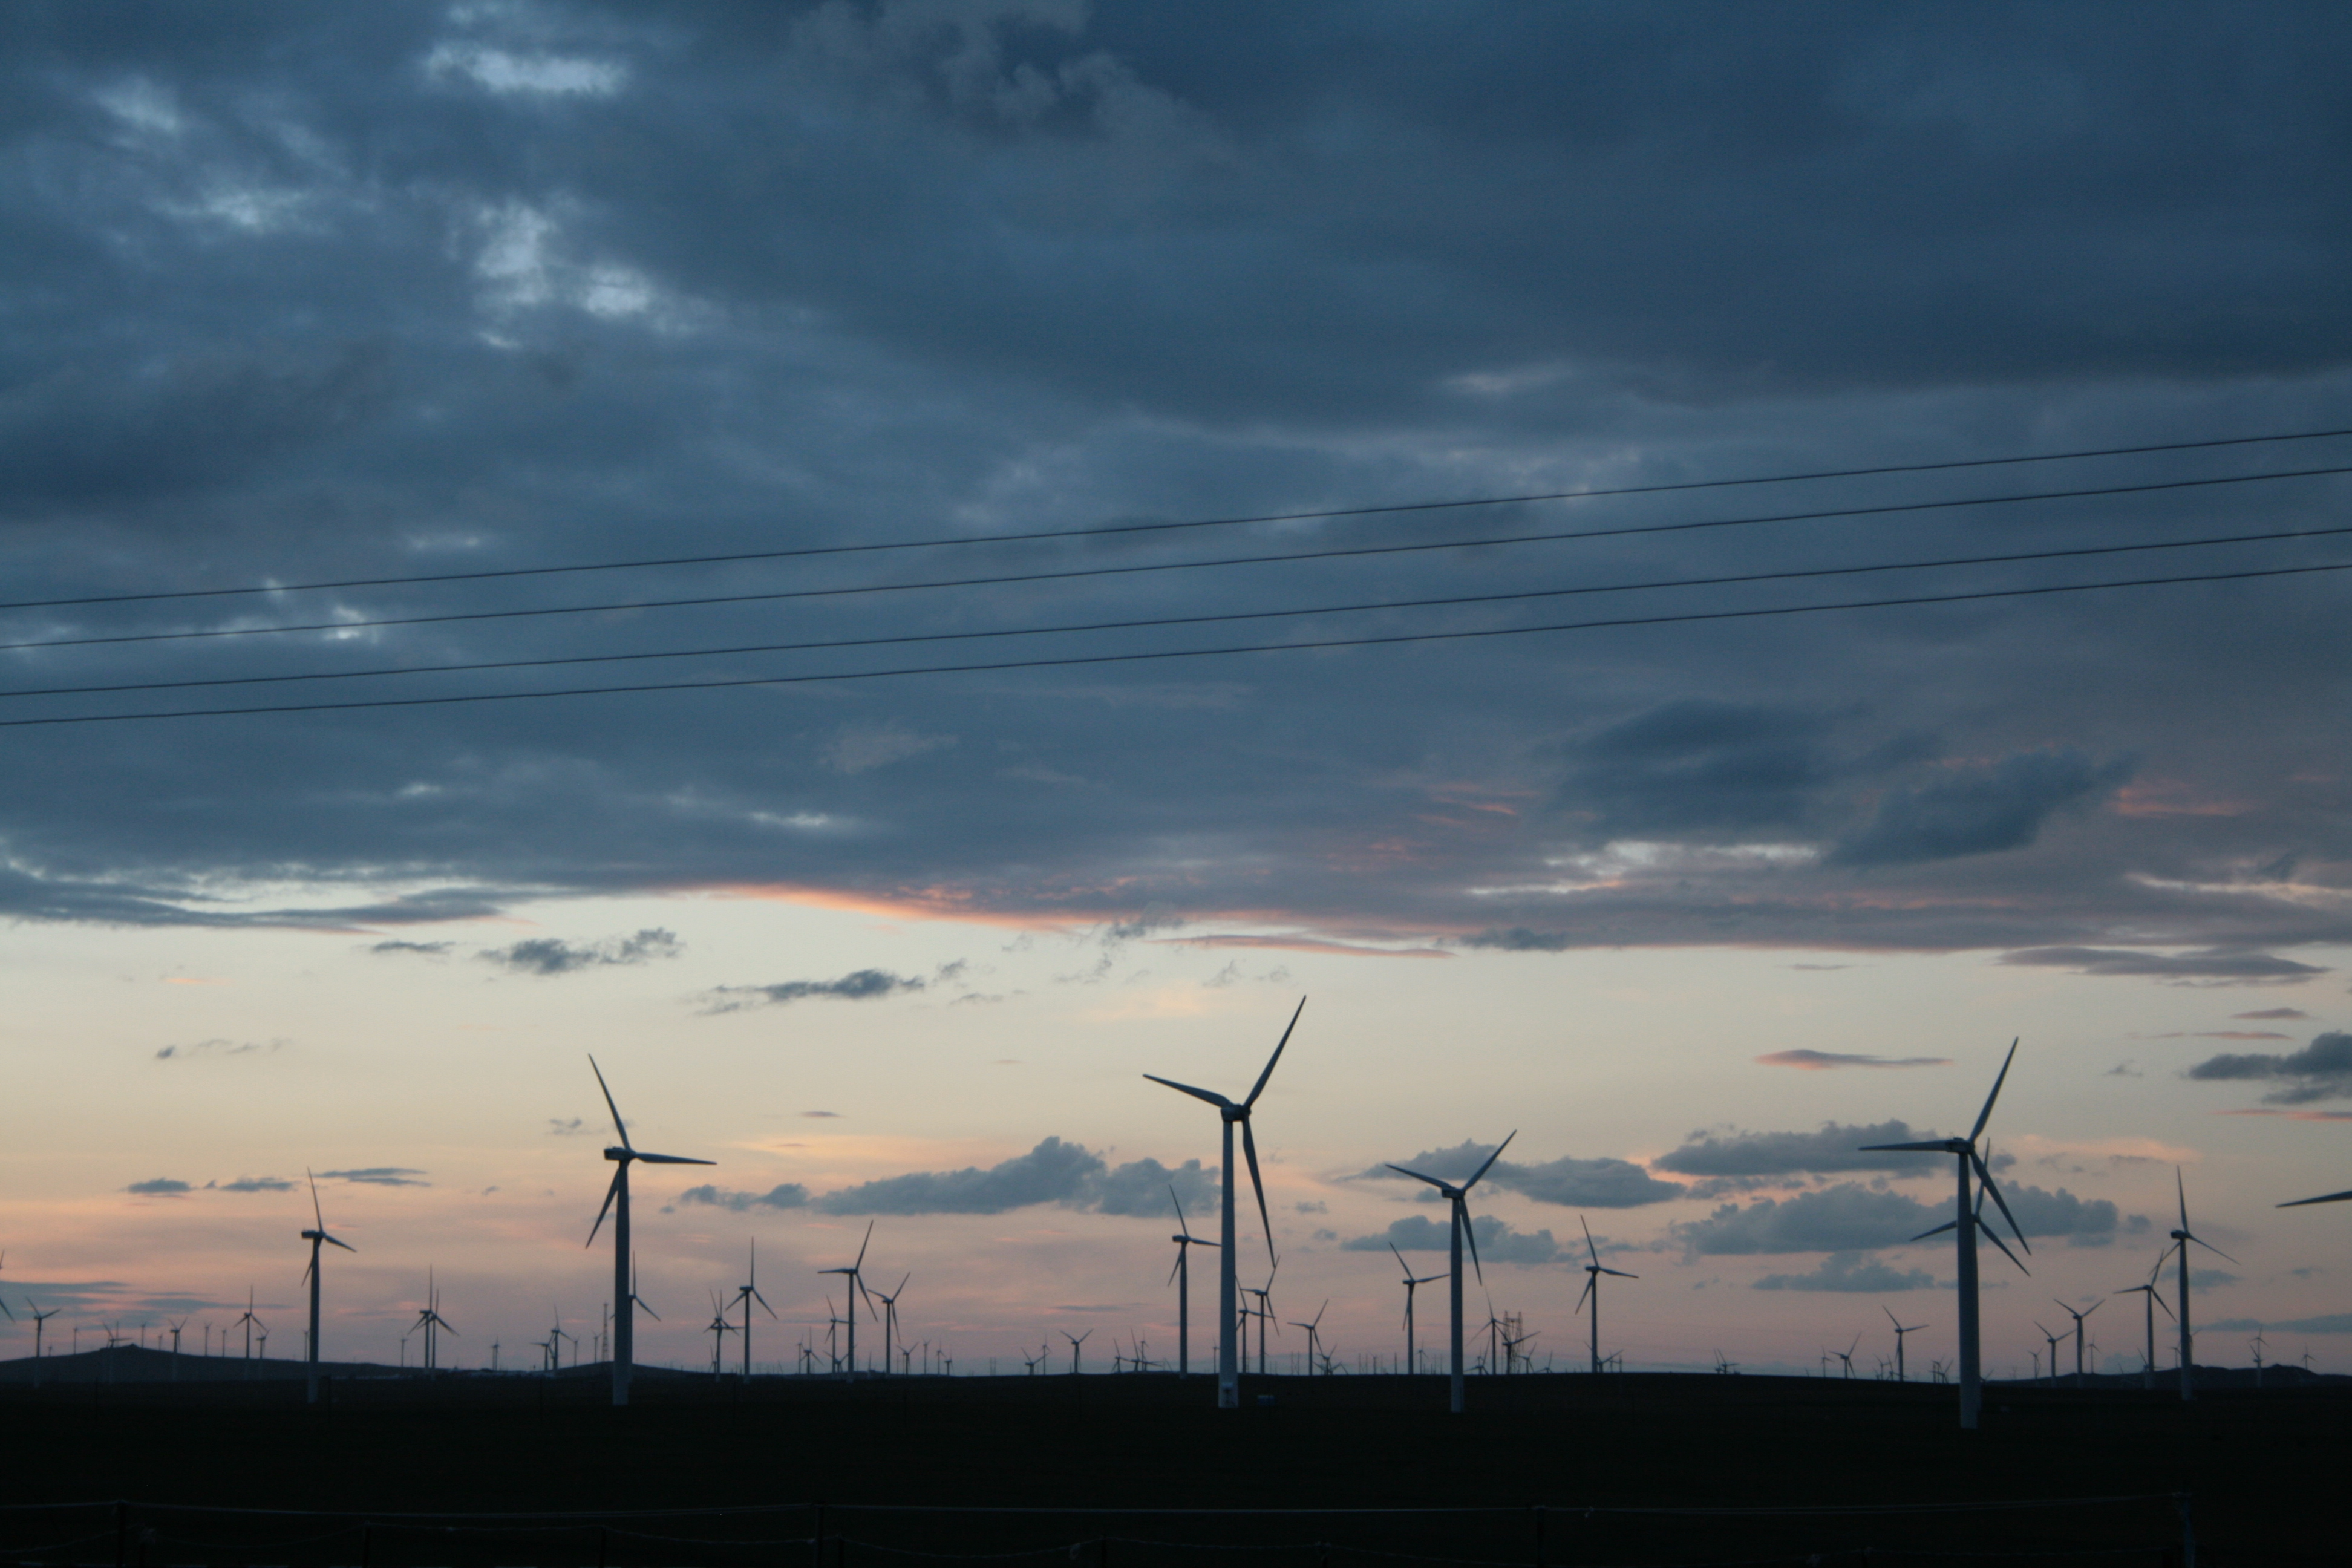
\includegraphics[width=\paperwidth, height=1.1\paperheight]{aeromongolia.JPG}};}
% \begin{frame}{RE in the electricity system}
% \begin{alertblock}  
% \begin{itemize}
%   \item{\textcolor{black}{Demand and supply need to be \textbf{\alert{balanced}}}.}
%   \item{\textcolor{black}{Electricity systems are designed for centralized \alert{conventional power plants}}.}
%   \item{\textcolor{black}{\textbf{\alert{VRE}}: variable renewable energy}}
%   \end{itemize}
% \end{alertblock}
% \end{frame}
% }

 
%{
%\usebackgroundtemplate{\tikz\node[opacity=1, inner sep=0pt, outer sep=0pt]{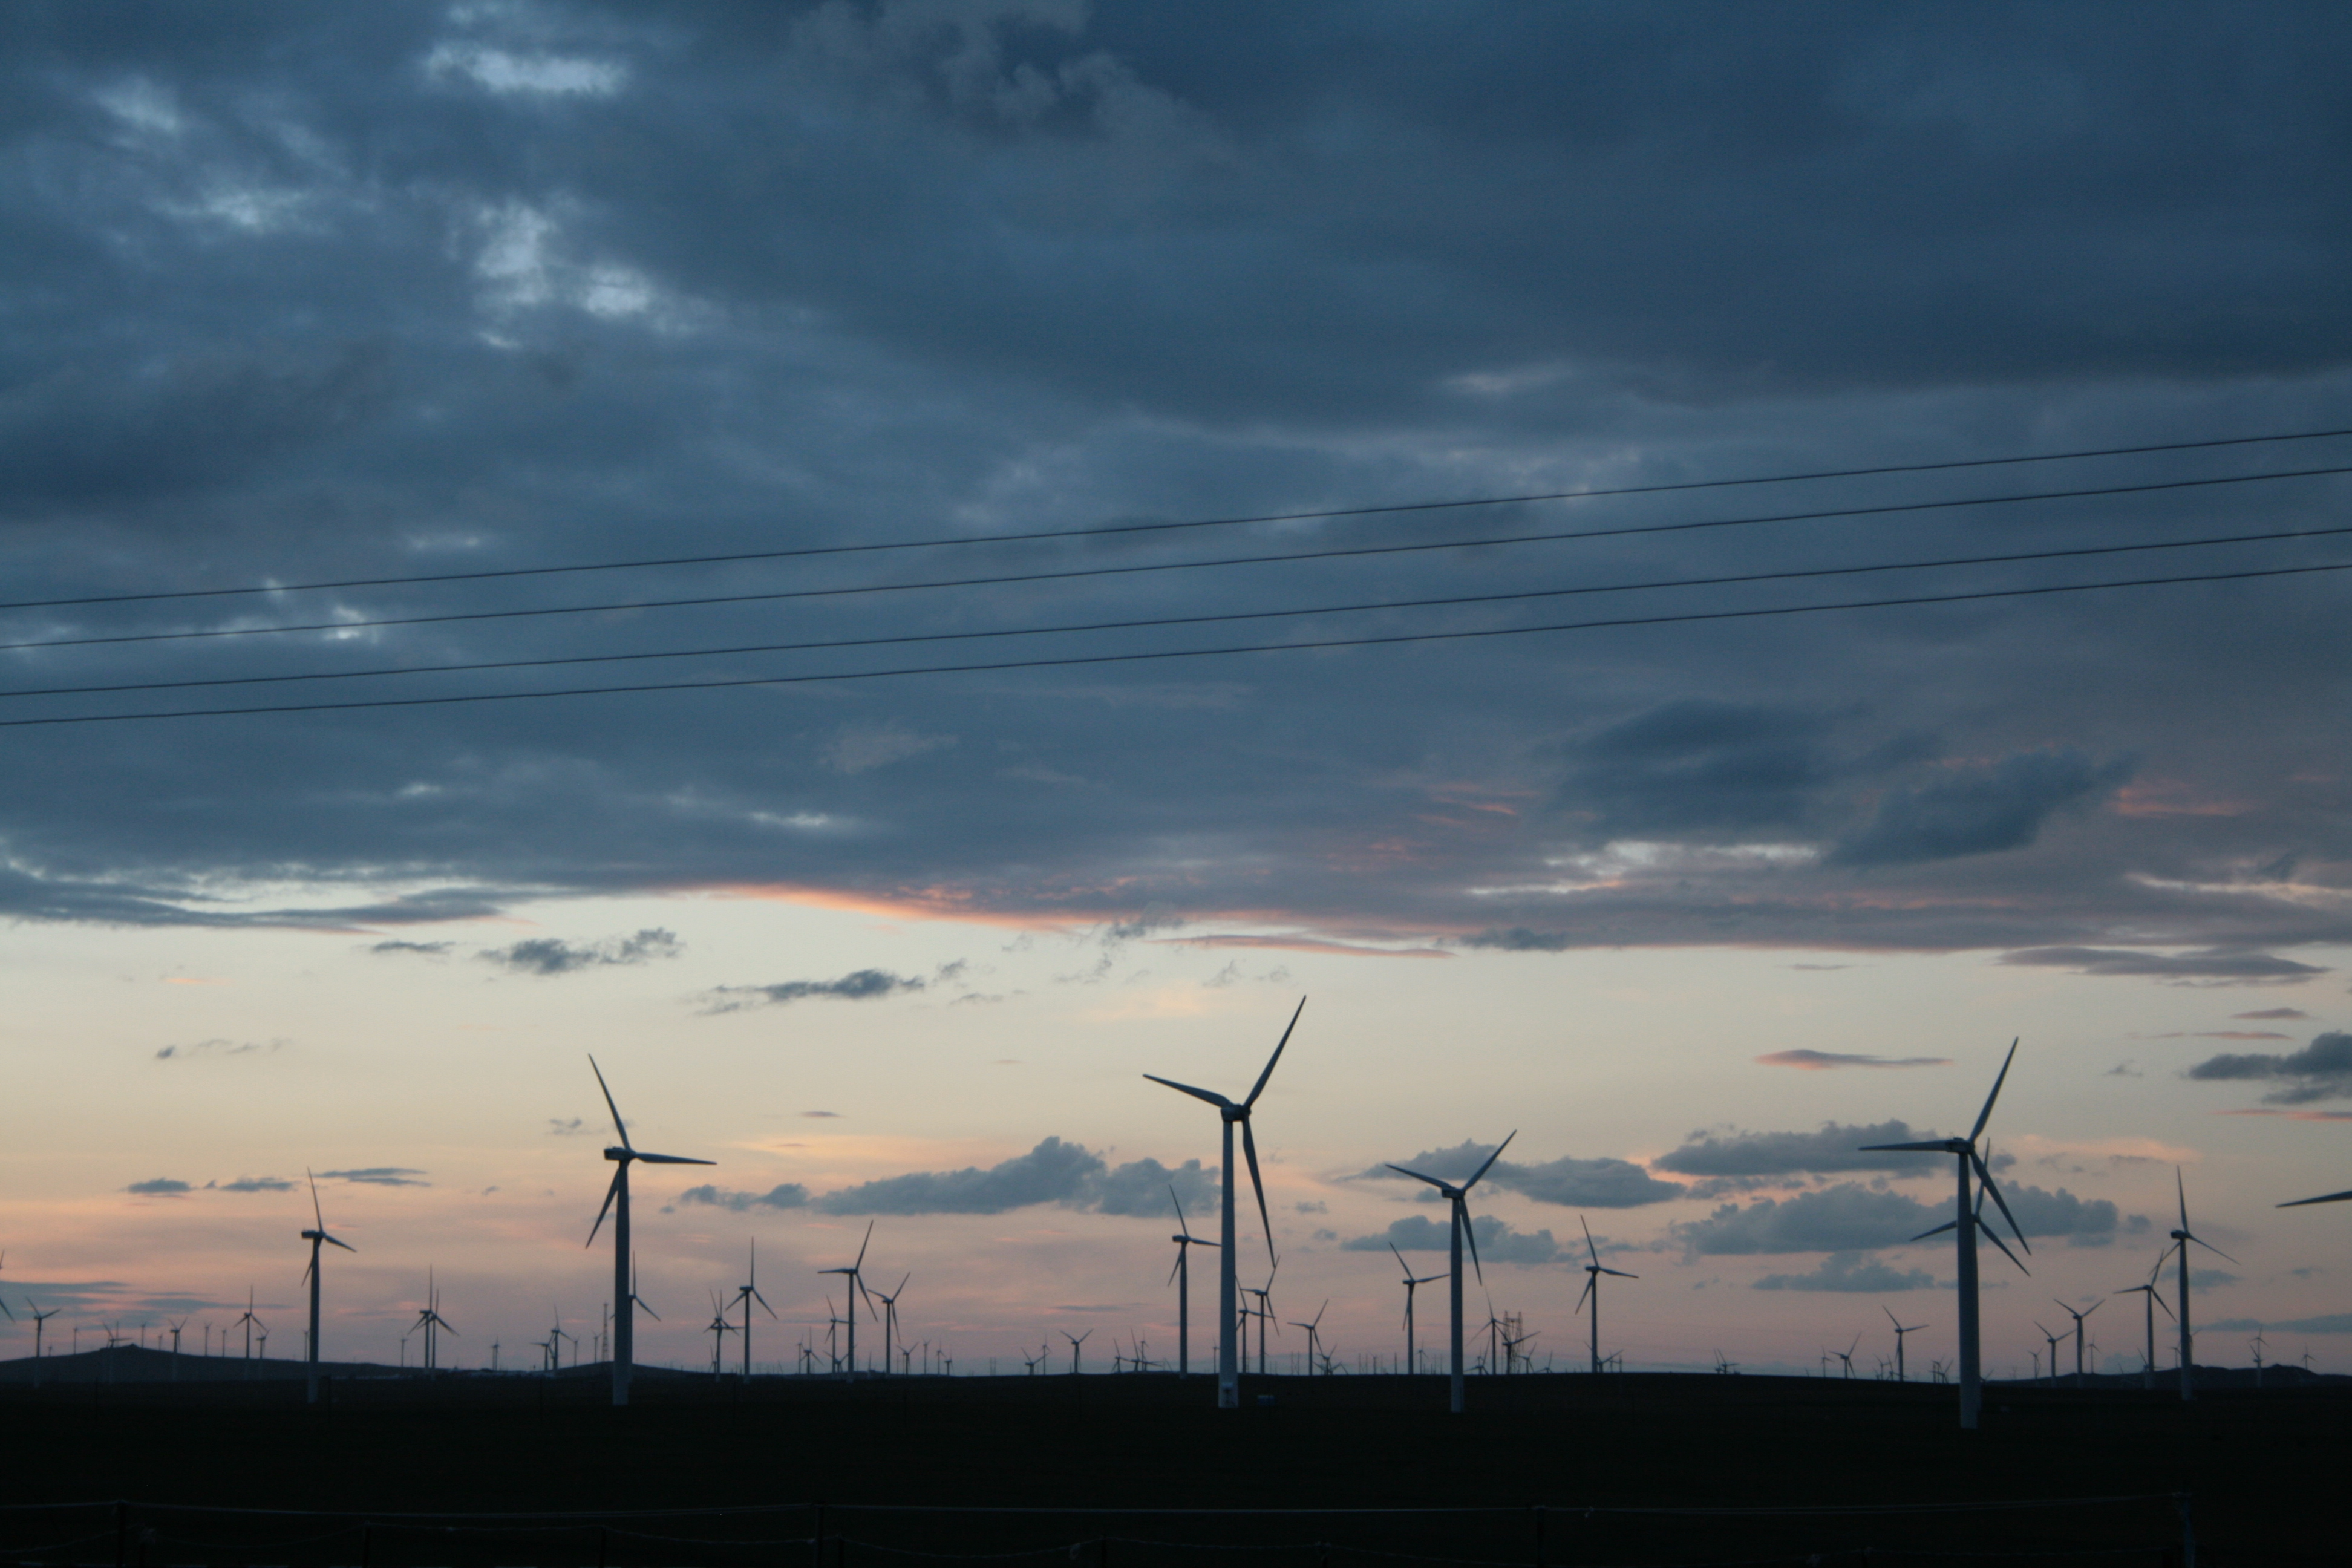
\includegraphics[width=\paperwidth, height=1.1\paperheight]{aeromongolia.JPG}};}
% \begin{frame}{RE in the electricity system}
% \begin{alertblock}
% \begin{itemize}  
%   \item Demand and supply need to be \alert{balanced}.
%   \item Electricity systems are designed for centralized \alert{conventional power plants}.
%   \item \alert{VRE}: variable renewable energy.
% \end{itemize}
% \end{alertblock}  
% \end{frame}
%}

% {
% \usebackgroundtemplate{\tikz\node[opacity=1, inner sep=0pt, outer sep=0pt]{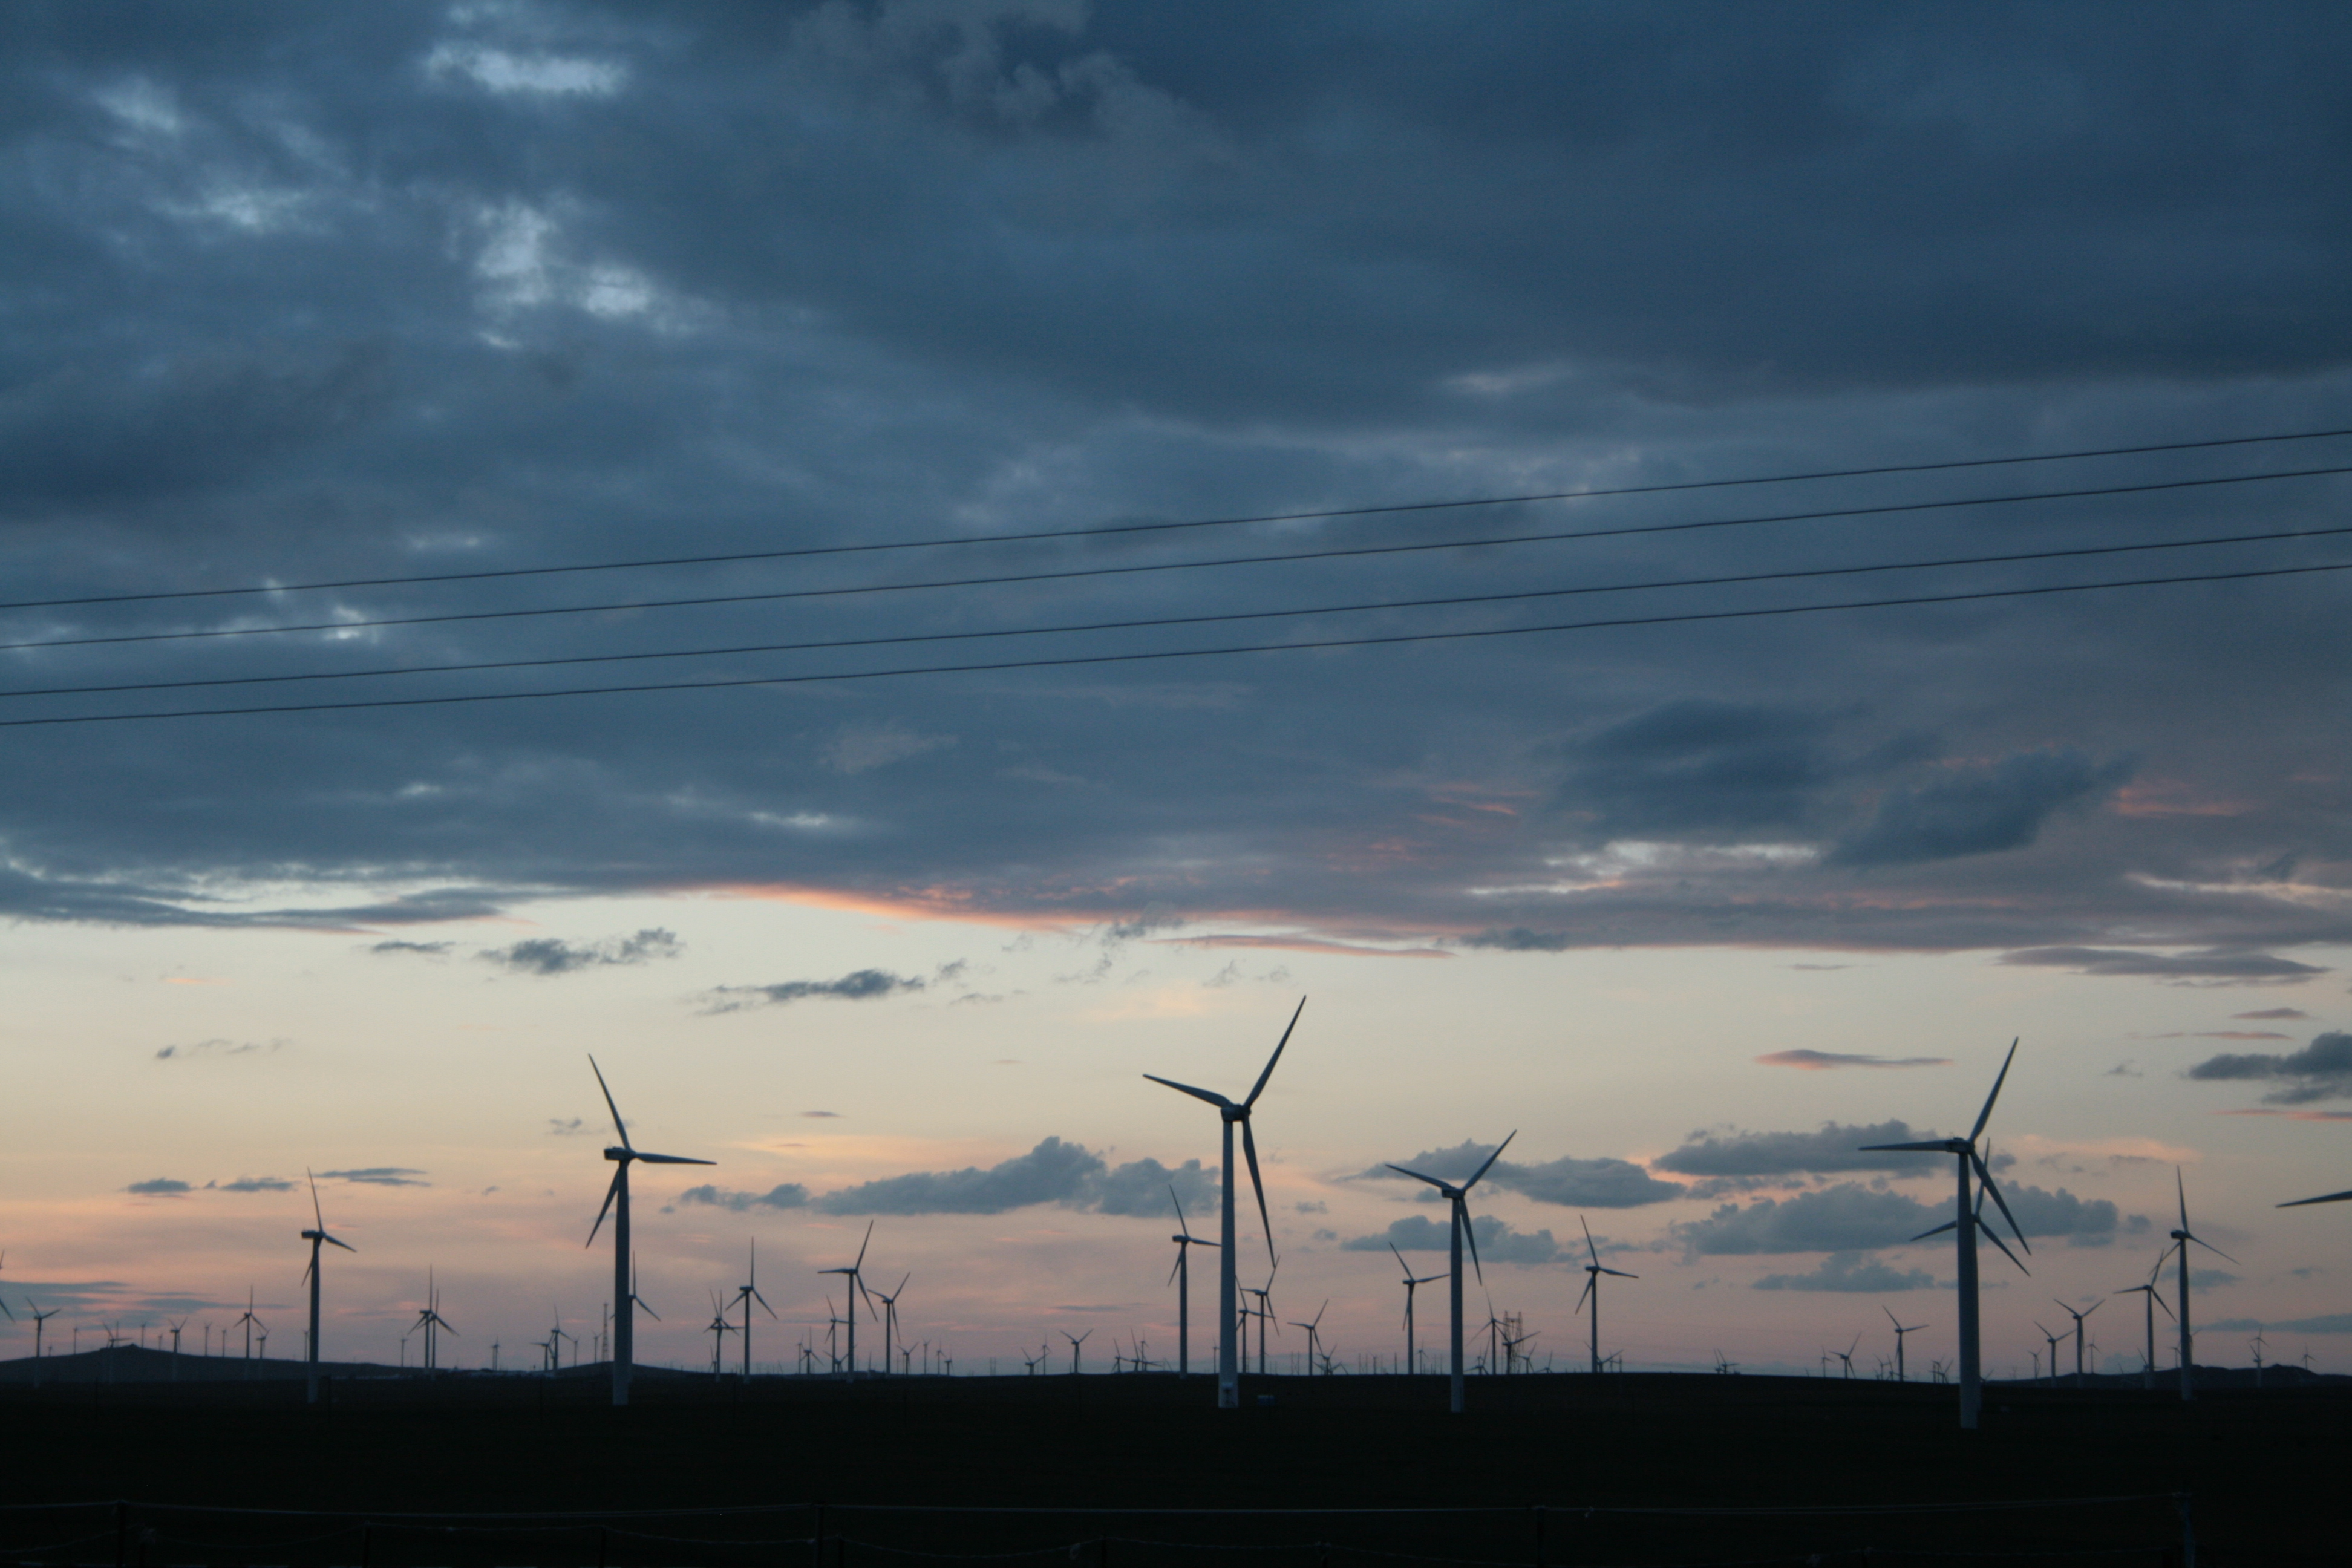
\includegraphics[width=\paperwidth, height=1.1\paperheight]{aeromongolia.JPG}};}
% \begin{frame}{RE in the electricity system}
% \end{frame}
% }

% {
% \usebackgroundtemplate{\tikz\node[opacity=1, inner sep=0pt, outer sep=0pt]{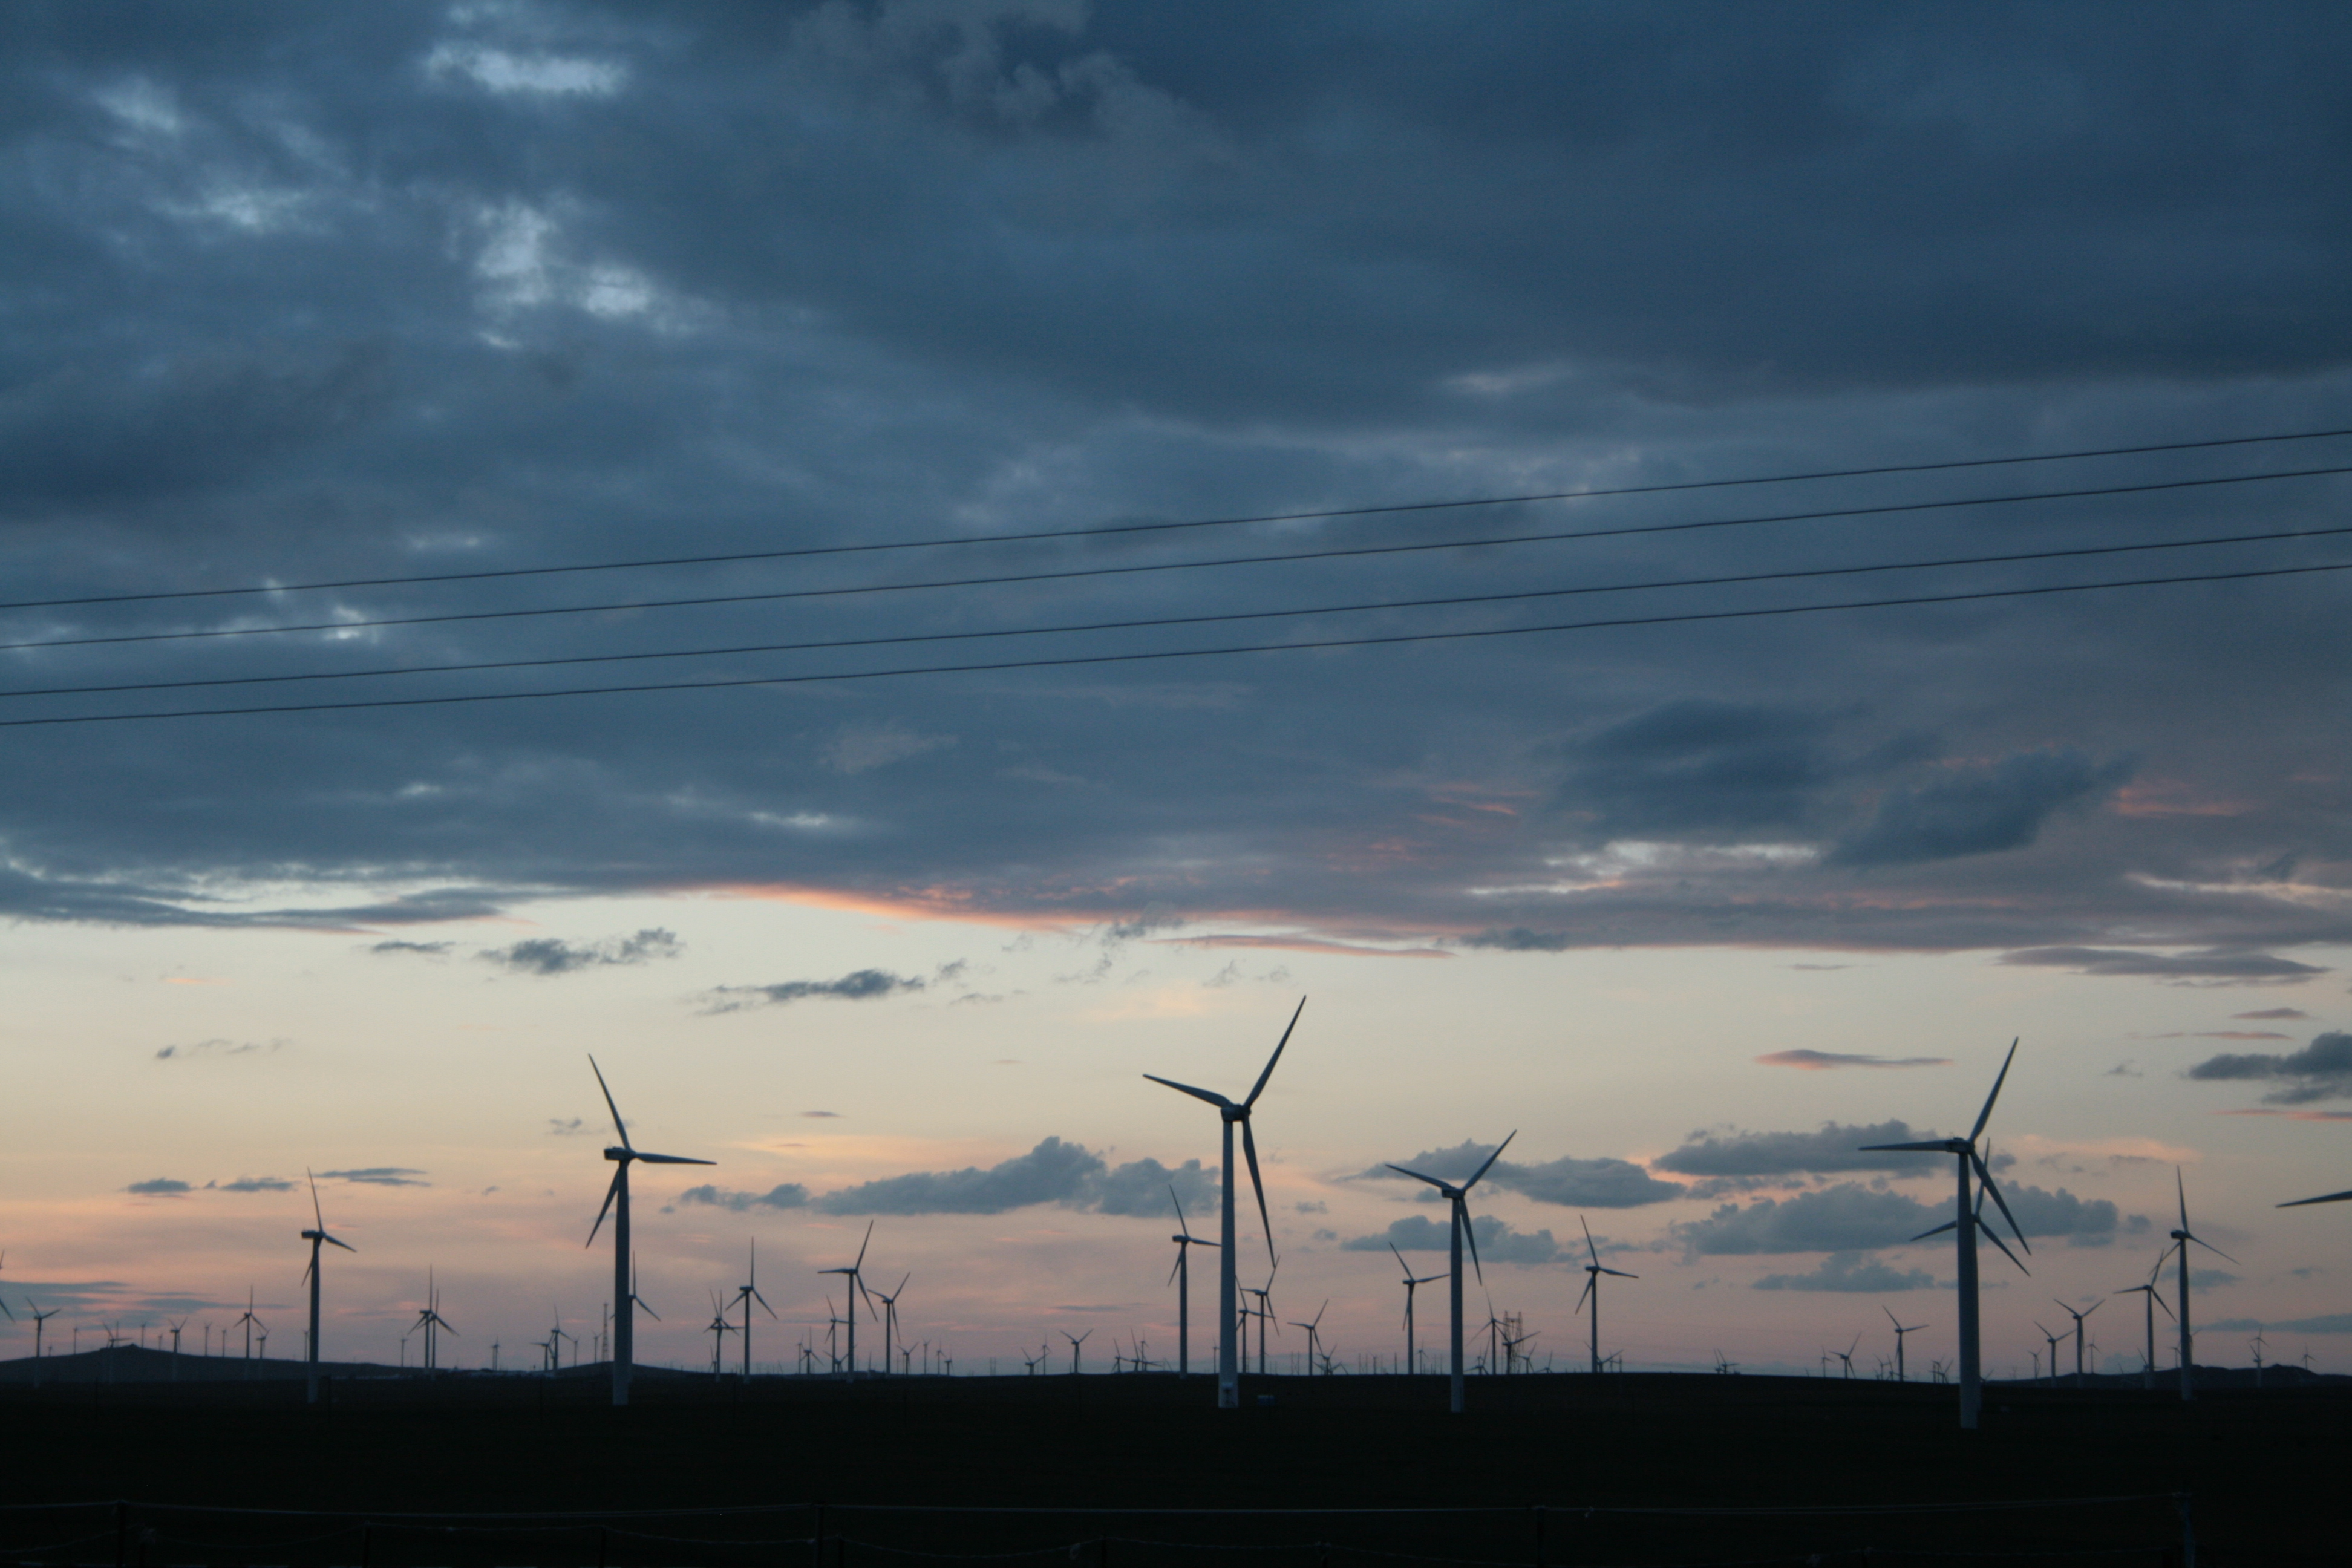
\includegraphics[width=\paperwidth, height=1.1\paperheight]{aeromongolia.JPG}};}
% \begin{frame}{RE in the electricity system}
%   \begin{beamercolorbox}[wd={11cm}, ht={3.2cm},
% sep=3mm,center,rounded=true,
% shadow=false]{postit}
% \begin{itemize}  
%   \item Demand and supply need to be \alert{balanced}.
%   \item Electricity systems are designed for centralized \alert{conventional power plants}.
%   \item \alert{VRE}: variable renewable energy.
%   \end{itemize}
% \end{beamercolorbox}
% \end{frame}
% }

\begin{frame}{RE in the electricity system}
\centering\Large {Electricity systems features:}
\small{  \begin{itemize}  
  \item <2->Demand and supply need to be \textbf{\alert{balanced}}.
  \item <3->Electricity systems are designed for centralized \alert{conventional power plants}.
  \item <4->\textbf{\alert{VRE}}: variable renewable energy.
  \end{itemize}}
\centering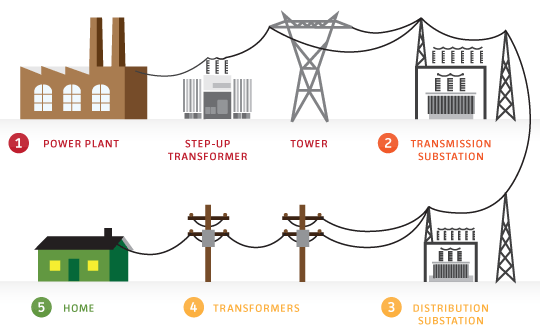
\includegraphics[width=0.5\textwidth]{system.png}
\end{frame}




\begin{frame}{VRE: variable renewable energy}
%\centering\Large {VRE: variable renewable energy}
\begin{columns}
  \begin{column}{0.55\textwidth}
\small{\begin{itemize}
%  \item RE variable in space and time
 \item<2-> \textbf{\alert{Intermittency}}: not synchronized with the demand
  \item<3-> Need of forecasting, plannification and/or storage
  \item<4-> Variations \textbf{from short to long scales}\\ (weather to climate)
    \begin{itemize}
    \item \alert{short}: operation
    \item \alert{medium}: planning, maintenance
    \item \alert{long}: resource assessment, financing, planning
  \end{itemize}    
\end{itemize}}
\end{column}
\begin{column}{0.6\textwidth}
  \centering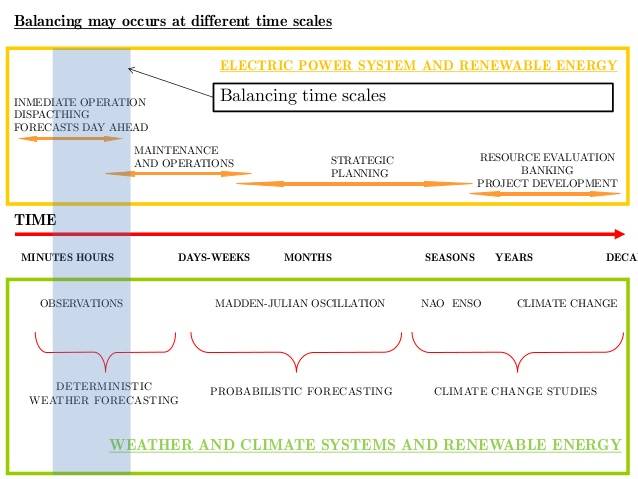
\includegraphics[width=1\textwidth]{timescales.jpg}
\end{column}
\end{columns}
%\centering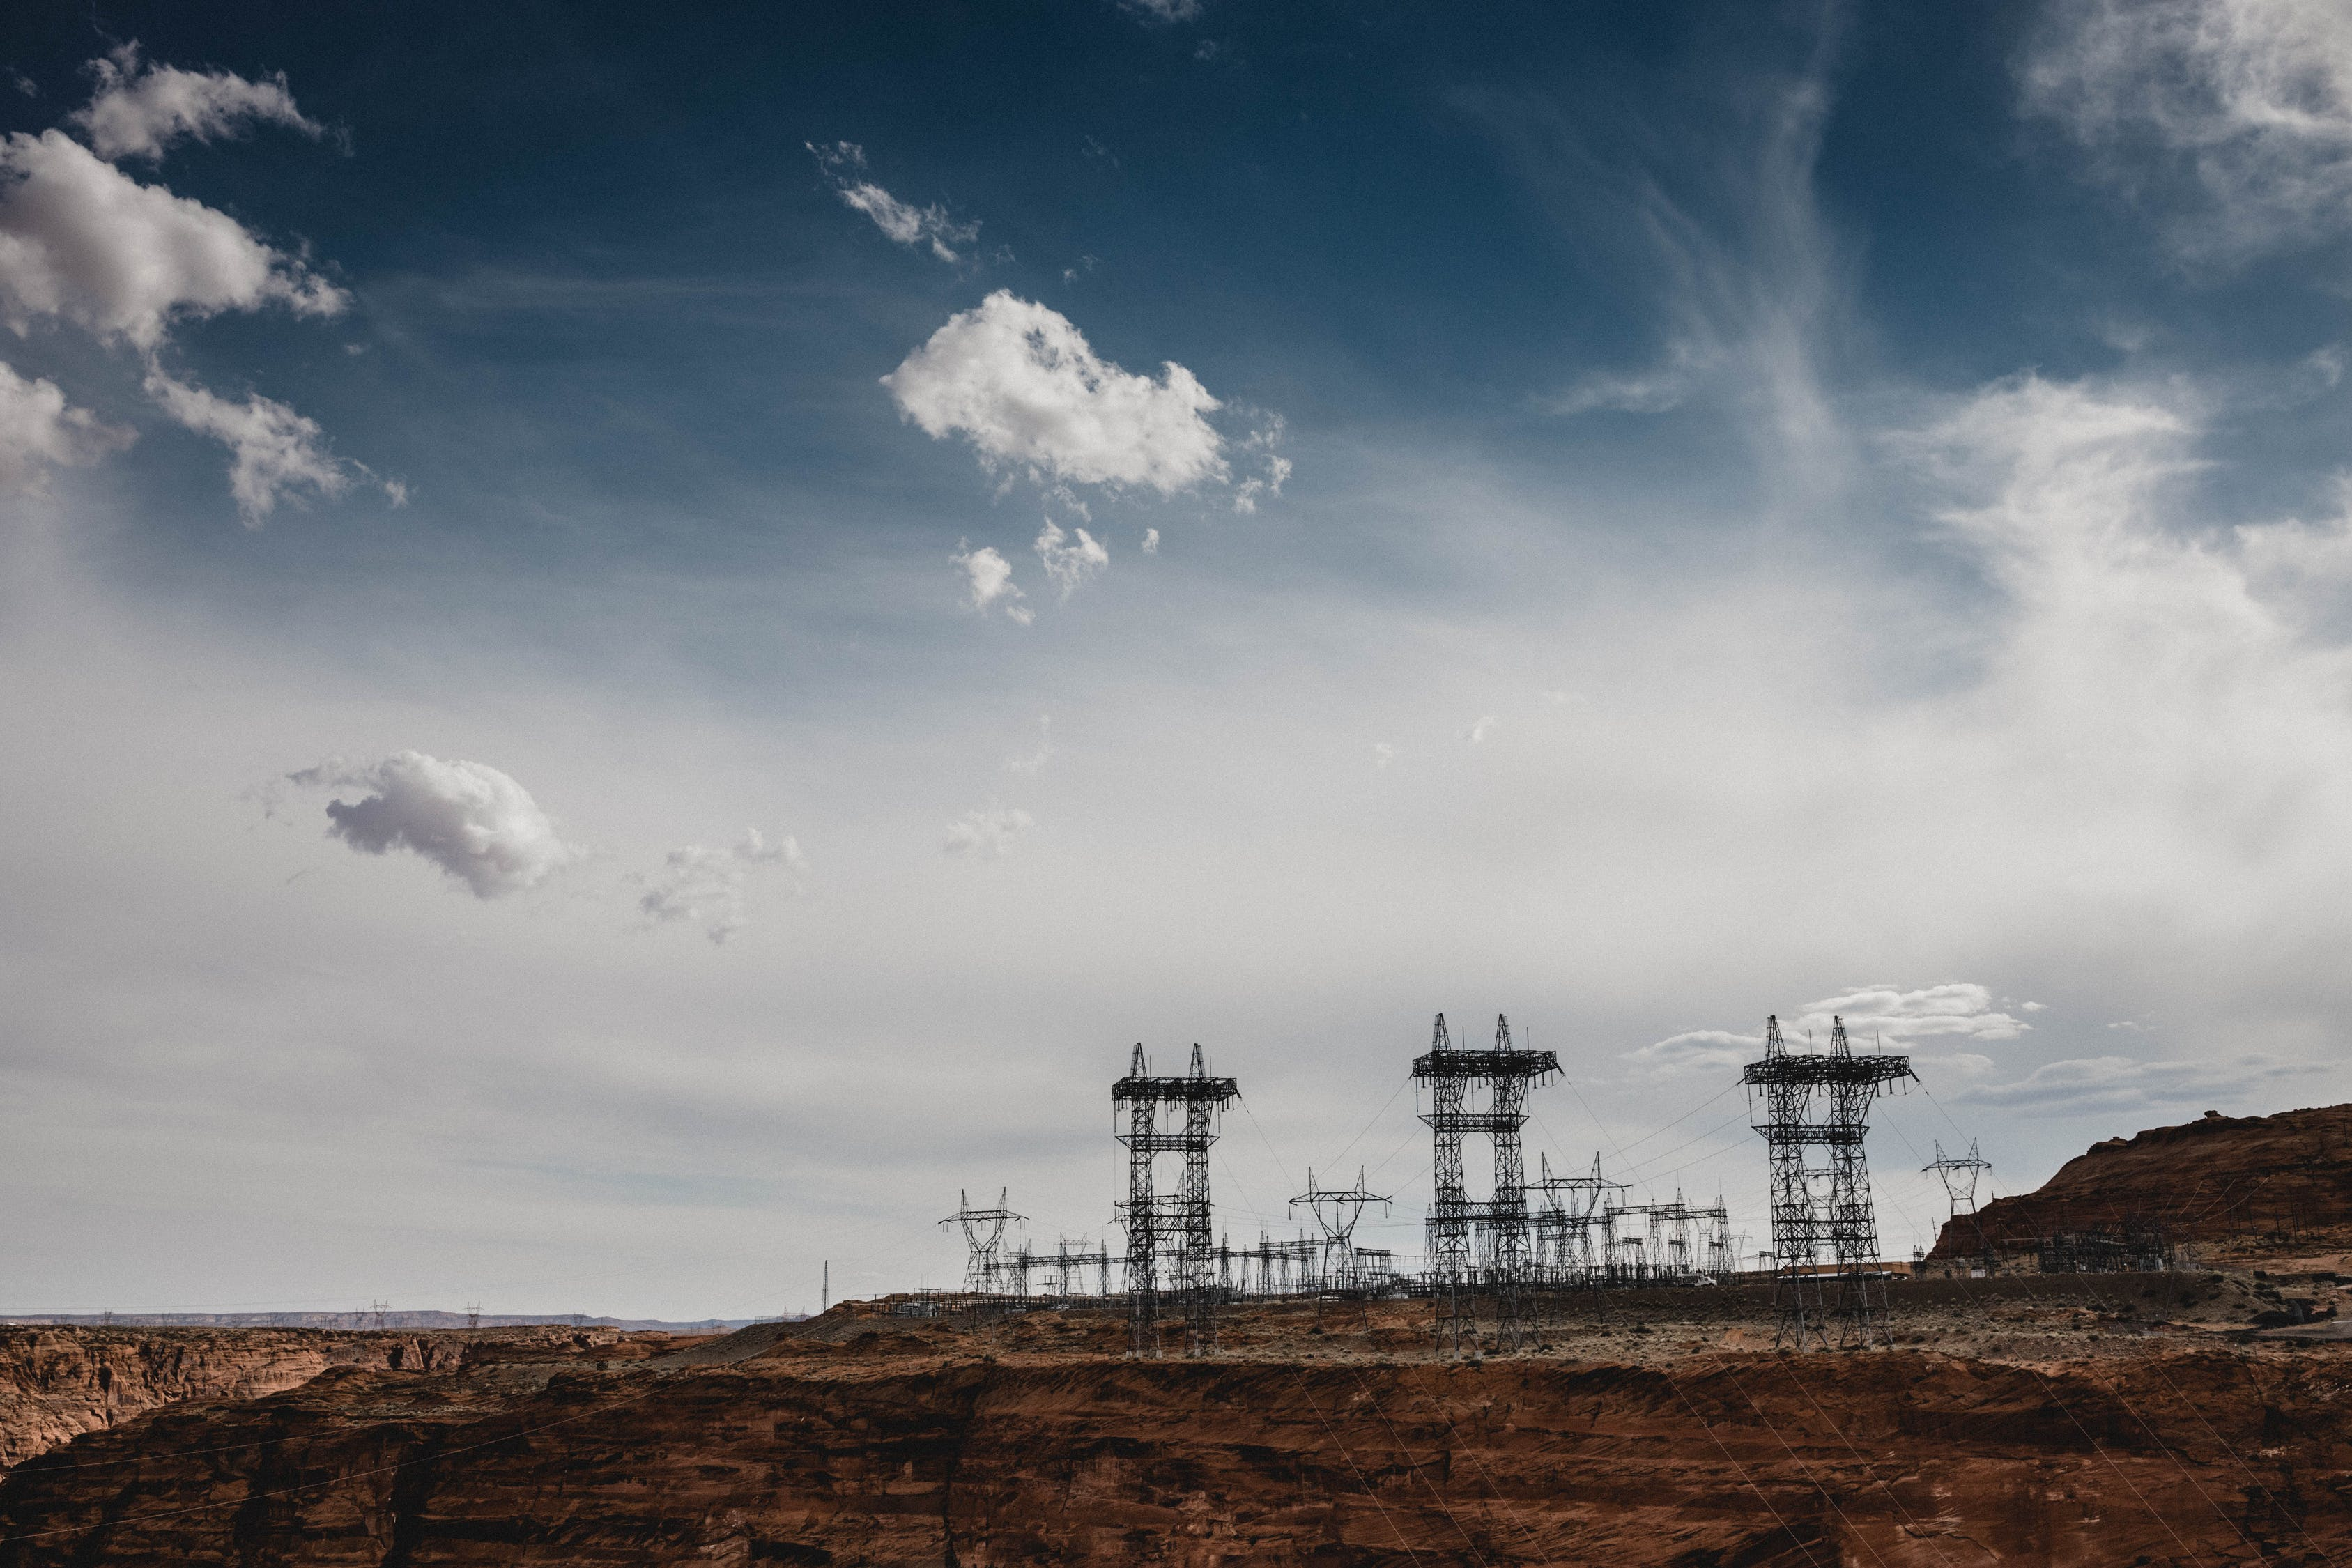
\includegraphics[width=0.5\textwidth]{powerline3.jpeg}
% \end{column}
% \begin{column}{0.3\textwidth}
% \end{column}
% \end{columns}
\end{frame}

\begin{frame}{Long scales: links between climate and renewables}
\centering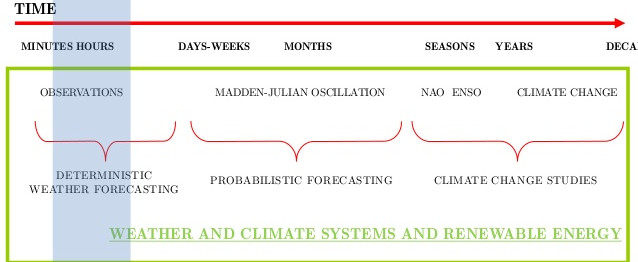
\includegraphics[width=0.8\textwidth]{timescales2.jpg}
\end{frame}


% {
% \usebackgroundtemplate{\tikz\node[opacity=0.5, inner sep=0pt,outer sep=0pt]{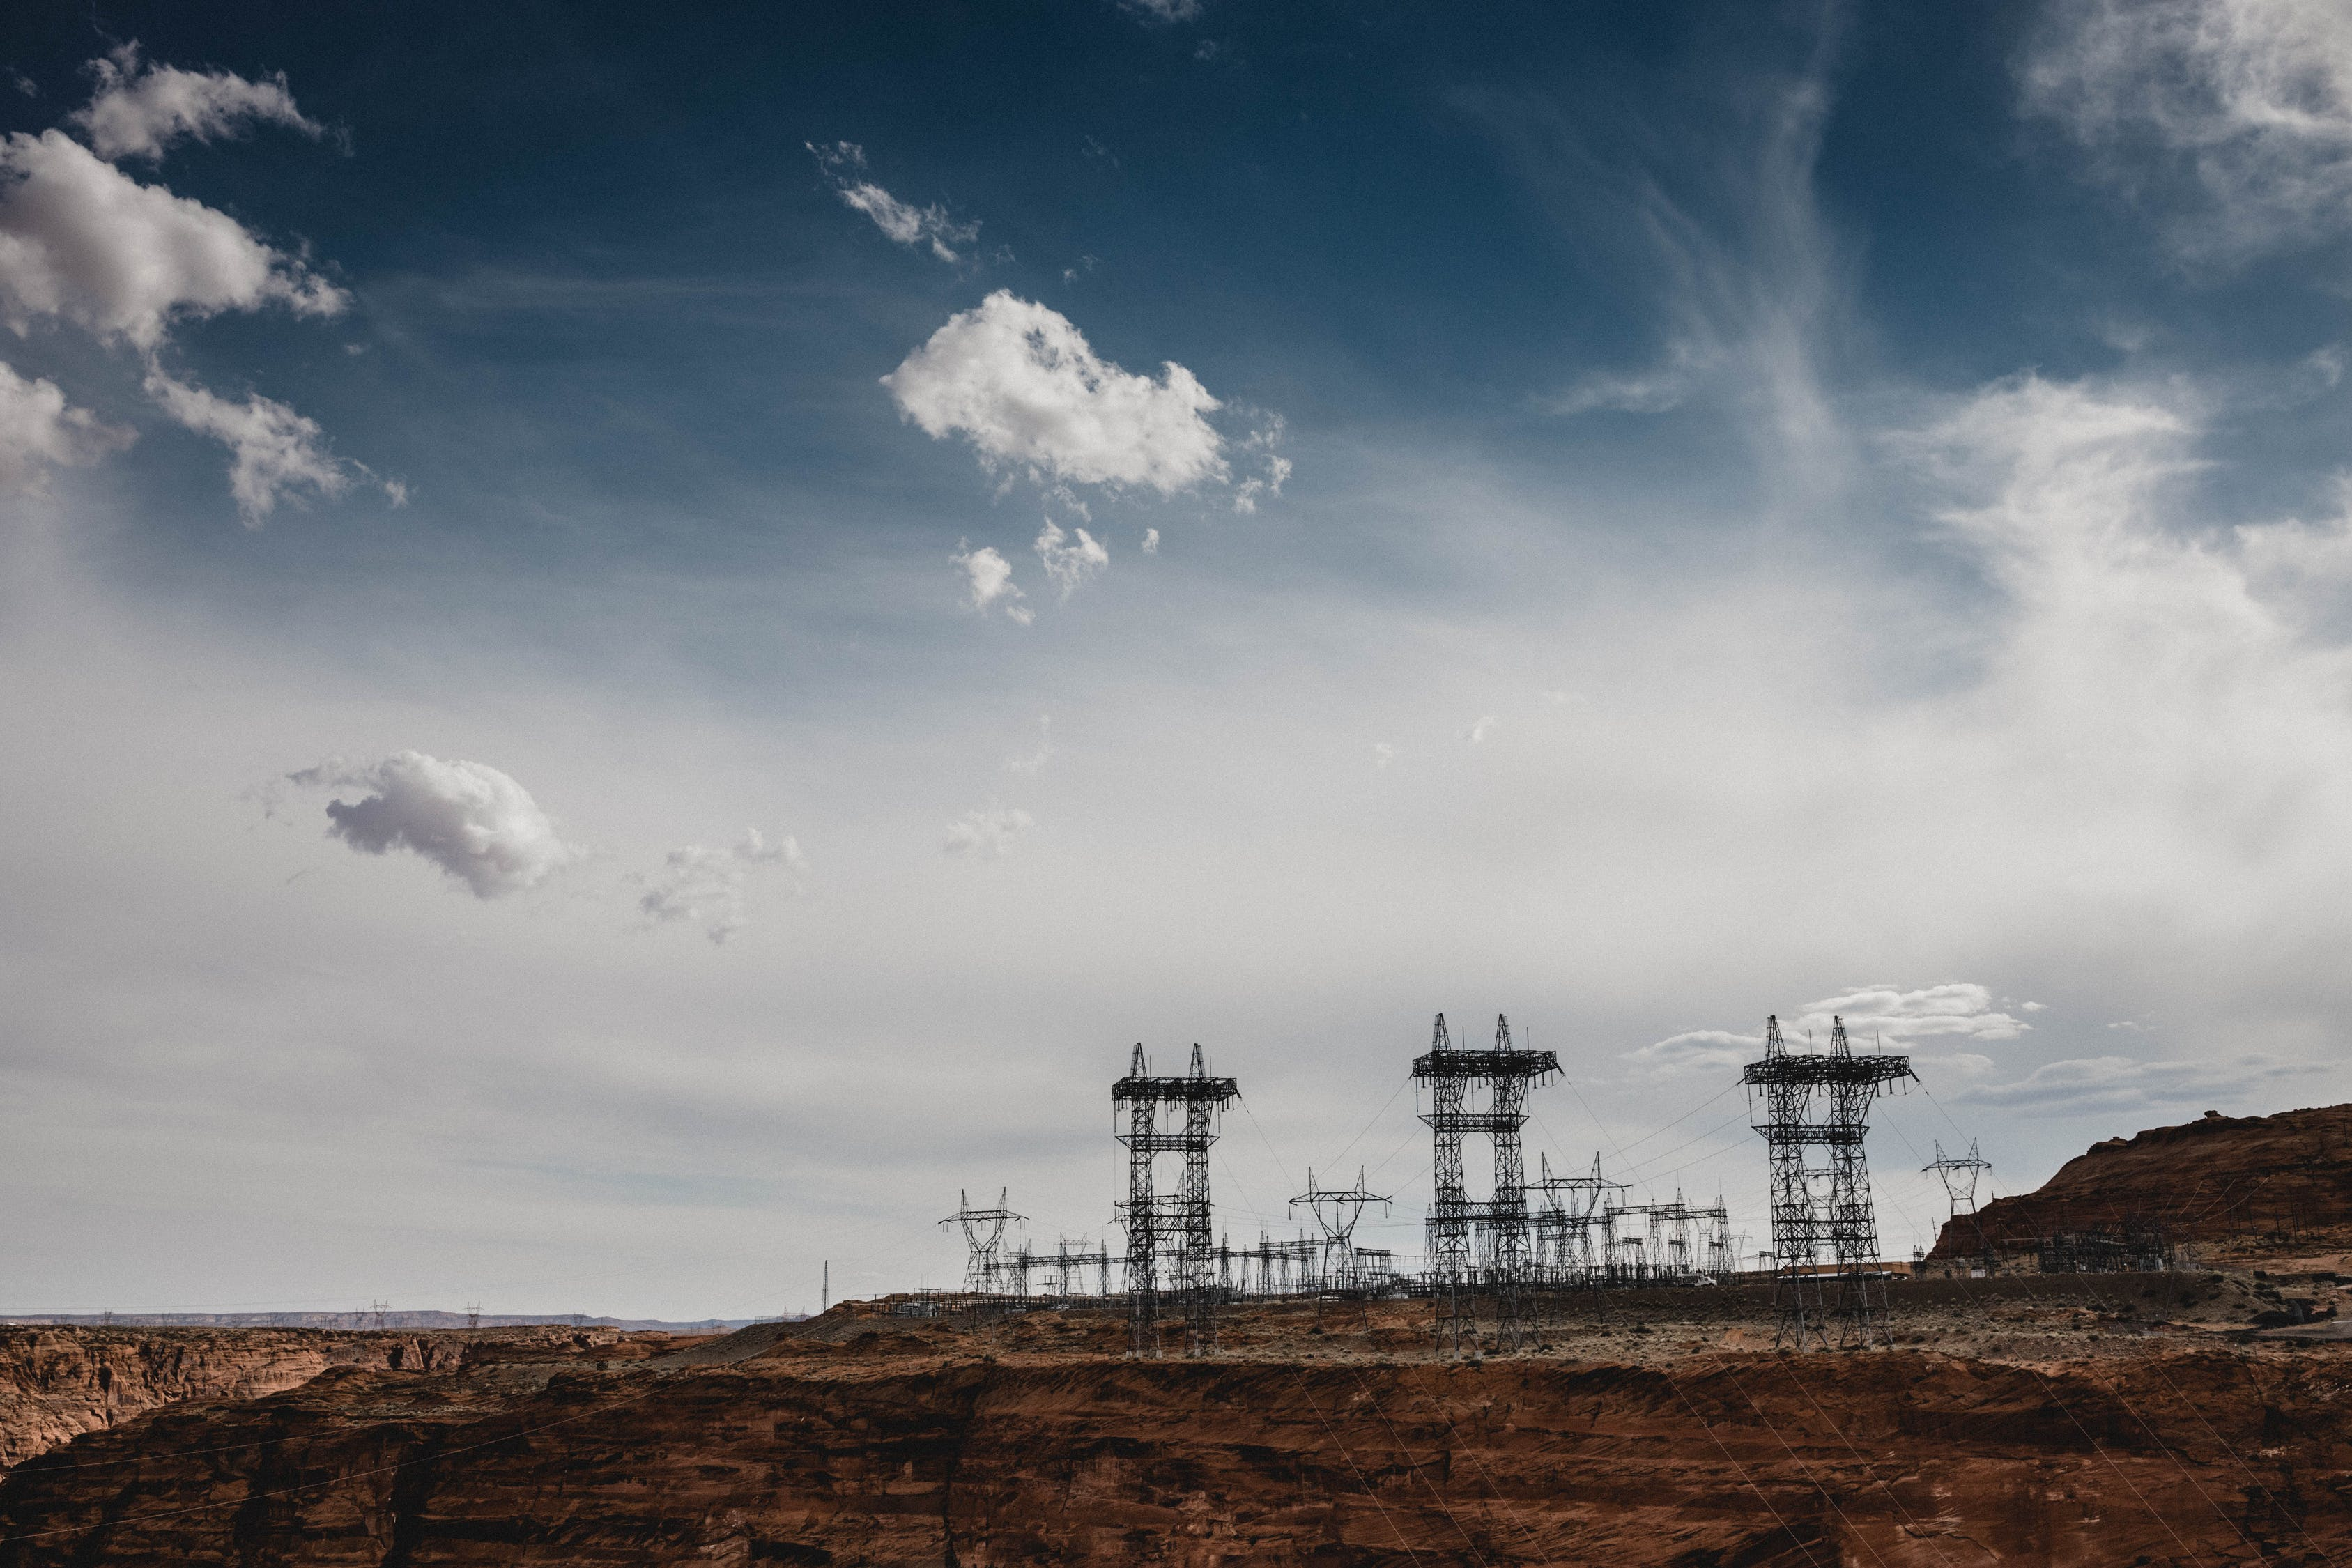
\includegraphics[width=\paperwidth, height=\paperheight]{powerline3.jpeg}};}
% \begin{frame}{VRE}
% \Large{\centering{Need for long-term projections of \textbf{\alert{resource and PV potential}}\\}}
% \vspace{1\baselineskip}
%   \begin{columns}
%    \begin{column}{0.6\textwidth}
%   \begin{itemize}
%   \item RE variable in space and time
%   \item Not syncrinized with the demand
%   \item Need of forecasting, plannification, storage
%   \item Variations from short to long-scales
%     \begin{itemize}
%     \item short: operation
%     \item medium: planning, maintenance
%     \item long: resource assessment, financing, planning
%   \end{itemize}    
%   \end{itemize}
%  \end{column}
%  \begin{column}{0.3\textwidth}
%  \end{column}
%  \end{columns}
% \end{frame}
% }

\begin{frame}[plain]{Variability sources on PV}
  \begin{itemize}
  \item Solar resource is \textbf{variable} from short to long-term time scales. %Composition of the atmosphere defines the amount of energy that reaches the PV generator surface.
  \item  Main drivers of solar resource variability are \textbf{cloudiness} and \textbf{aerosols}.
\end{itemize}
    % \begin{columns}
    % \begin{column}{0.4\textwidth}
    %   \small{The \textbf{\alert{Euro-Mediterranean area}} is influenced by aerosols from different sources. They have an impact on its climate. {\tiny({\textit{Nabat et al. 2015, Climate Dynamics})}}\\
    %     %\vspace{0.5\baselineskip}
    %     \small{They \textbf{impact} spatiotemporal variability of \textbf{PV production}.\\ {\tiny({\textit{Gutiérrez et al. 2018, Solar Enery}}) }\\}
    %             \vspace{0.5\baselineskip}
    %     \small{From the Euro-CORDEX ensemble, \textbf{few RCMs} include \textbf{aerosols evolution} in their scenario simulations.}
    % \end{column}
    % \begin{column}{0.5\textwidth}
       \begin{figure}
        \centering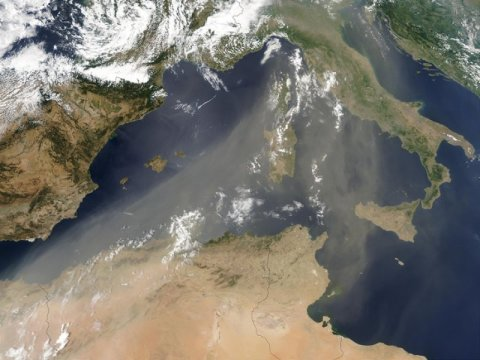
\includegraphics[scale=0.3]{ImageMODIScreditNASA}
        \centering\caption{Image from July 16th, 2003. MODIS. Credit:NASA}
\end{figure}
%\end{column}
%\end{columns}    
\end{frame}

\begin{frame}[fragile]{INTRODUCTION}
\Large{\centering{Need for long-term projections of \textbf{\alert{resource and PV potential}}\\}}
\vspace{1\baselineskip}
\small{Previous studies show a \textbf{discrepancy} between \textbf{GCMs} and \textbf{RCMs} surface solar radiation (SSR) over Europe:\\}
\begin{itemize}
     \item \alert{Increase} projected by GCMs {\tiny(\textit{Wild et al. 2015, Solar Energy})}.
     \item \alert{Decrease} projected by RCMs {\tiny(\textit{Jerez et al. 2015, Nature Communications})}.
     \end{itemize}
   % \textbf{Variabilidad estacional} muy marcada.
%     \end{column}
%     \begin{column}{0.4\textwidth}
%       \begin{figure}
%         \centering\includegraphics[scale=0.25]{mapa}
% \caption{Nabat 2016}
% \end{figure}
% \end{column}
\end{frame}

\section{Objectives and methodology}

\begin{frame}[fragile]{OBJECTIVE}
  \begin{itemize}
  \item {\Huge{\alert{1}}} To illustrate the \textbf{inconsistency} between \textbf{GCM} and \textbf{RCM} projections and to attribute it to missing aerosols forcing. 
    \vspace{1.5\baselineskip}
    \item {\Huge{\alert{2}}} To \textbf{deliver future projections of PV} potential production over Europe.
    \end{itemize}
 % \begin{alertblock}{RCM simulations from Euro-CORDEX}
%   \begin{itemize}
%   \item SSR from historical and RCP8.5.
%   \item Simulations grouped by forcing GCM and aerosols representation.
%   \end{itemize}
% \end{alertblock}  
% \begin{alertblock}{solaR}
% Use of a parametric PV model. Implemented in R \tiny{(O. Perpiñán, 2013)}.
% \end{alertblock}
% \
\end{frame}

\begin{frame}[fragile]{METHODS}
  \begin{itemize}
  \item {\Huge{\alert{1}}} To illustrate the \textbf{inconsistency} between \textbf{GCM} and \textbf{RCM} projections and to attribute it to missing aerosols forcing.
    \vspace{1\baselineskip}
    \begin{itemize} 
    \item Use of well-chosen groups of GCM-RCM within the \alert{Euro-CORDEX} ensemble. 
     \item \textbf{2021-2050} summer change in surface solar radiation, \alert{SSR}, with respect of a reference period: \textbf{1971-2000}. Use of \textbf{RCP8.5} scenario.
    \end{itemize} 
  \end{itemize}
  \vspace{1\baselineskip}
  \begin{table}
    {\small{
    \centering{\begin{tabular}[1\textwidth]{c|c|c}
      \toprule
      GCM & RCM & Aerosols \\
      \midrule 
                & CCLM4-8-17 & - \\
       CNRM-CM5 & \alert{ALADIN53} & Szopa et al.\\
                & RCA4 & -\\
      \midrule           
                & CCLM4-8-17 & - \\
      EC-EARTH  & \alert{RACMO22E} & Lamarque et al.\\
                & RCA4 & -\\
      \bottomrule
               \end{tabular}}
             \vspace{0.75\baselineskip}
             \caption{Groups of GCM-RCM used}
     \end{table}}}
\end{frame}


\begin{frame}[fragile]{METHODS}
  \begin{itemize}
  \item {\Huge{\alert{2}}} To \textbf{deliver future projections of PV} potential production over Europe.
  \end{itemize}
\begin{alertblock}{solaR}
\end{alertblock}
Parametric PV model. \textbf{SSR} from \textbf{RCM} as input -> POA and electrical performance. Implemented in R \tiny{(O. Perpiñán, 2013).
  \vspace{2\baselineskip}
      \begin{figure}
      \centering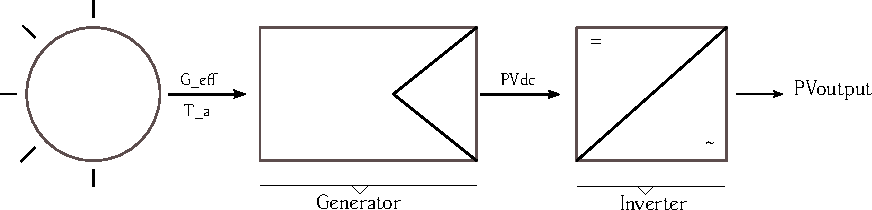
\includegraphics[scale=0.5]{pvsistem.pdf}
      \vspace{1\baselineskip}
      \centering\caption{Squeme of a PV generator.}
      \end{figure}
\end{frame}

\section{Results}
 
\begin{frame}[fragile]{SSR mean changes 2021-2050}
\vspace{1\baselineskip}
\begin{columns}
  \begin{column}{0.45\textwidth}
    \centering{\hspace{3\baselineskip}\LARGE{\textbf{GCM}}}
      \end{column}
      \begin{column}{0.7\textwidth}
        \hspace{5.4\baselineskip}{\LARGE{\textbf{RCM}}}
   \end{column}
   \end{columns}
    \begin{figure}
      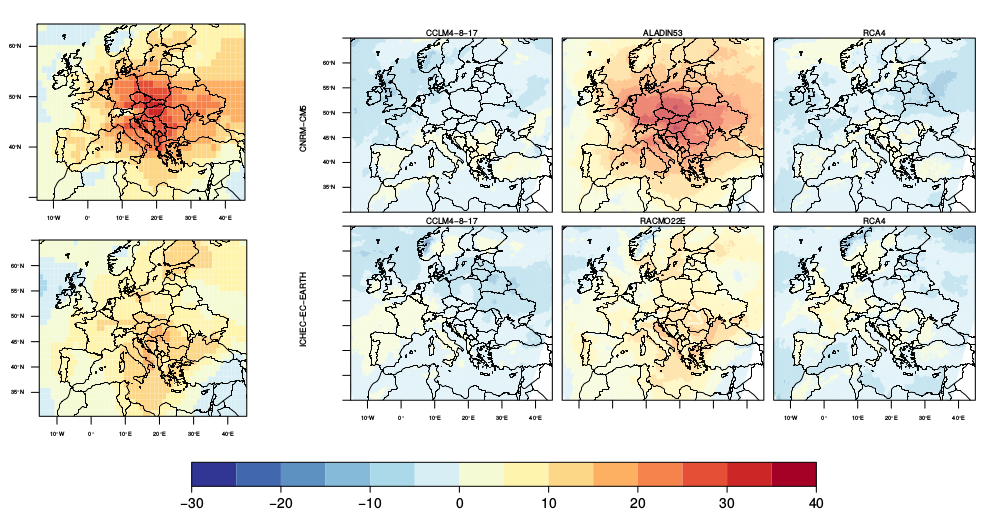
\includegraphics[scale=0.32]{ssr_gimp4.png}
        \centering\caption{SSR change (1971/2000)-(2021/2050) ($W/m^2$)}
      \end{figure}
\end{frame}

\begin{frame}[fragile]{SSR mean changes 2021-2050}
\vspace{0.5\baselineskip}
\begin{columns}
  \begin{column}{0.7\textwidth}
 \hspace{1.8\baselineskip}\LARGE{\textbf{GCM}}
   %    \end{column}
   %    \begin{column}{0.7\textwidth}
      \hspace{4\baselineskip}{\LARGE{\textbf{RCM}}}
   % \end{column}
   % \end{columns}
    \begin{figure}
      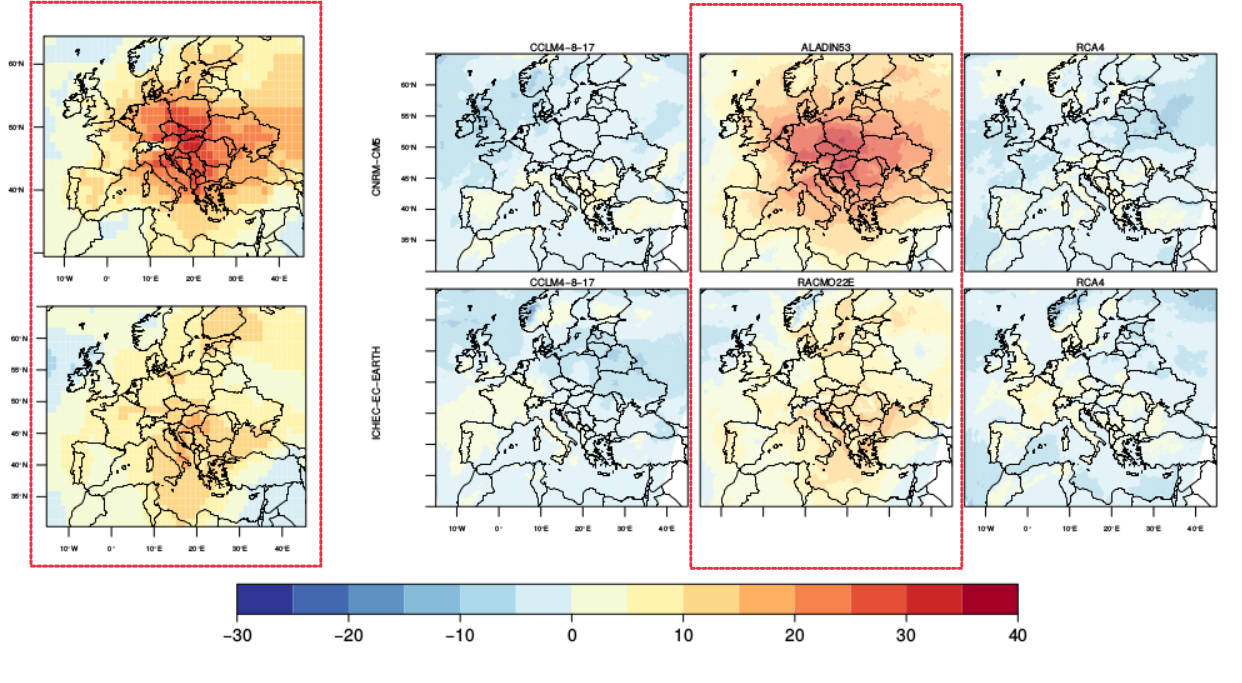
\includegraphics[scale=0.26]{ssr_gimp3.png}
        \centering\caption{SSR change (1971/2000)-(2021/2050) ($W/m^2$)}
    \end{figure}
  \end{column}
  \begin{column}{0.4\textwidth}
    \begin{itemize}
      \centering\item Only RCMs with evolving aerosols show the increase in SSR as GCMs.
    \end{itemize}
  \end{column}
  \end{columns}
\end{frame}
 
% \begin{frame}[fragile]{SSR mean changes 2021-2050}
% \vspace{0.5\baselineskip}
% \begin{columns}
%   \begin{column}{0.45\textwidth}
% \hspace{4\baselineskip}\centering{\LARGE{\textbf{GCM}}}
%       \end{column}
%       \begin{column}{0.7\textwidth}
%         \hspace{5.2\baselineskip}{\LARGE{\textbf{RCM}}}
%    \end{column}
%    \end{columns}
%     \begin{figure}
%       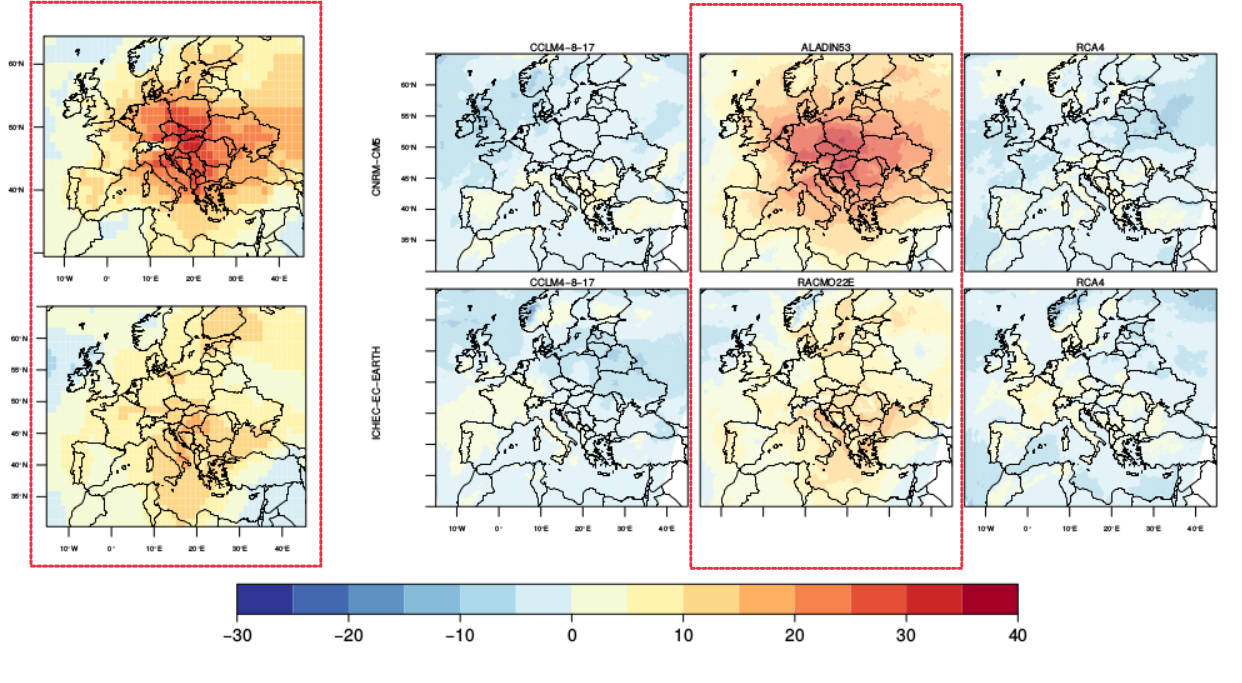
\includegraphics[scale=0.3]{ssr_gimp3.png}
%         %\centering\caption{SSR change (1971/2000)-(2021/2050) ($W/m^2$)}
%     \end{figure}
% %    \vspace{0.01\baselineskip}
%       \begin{itemize}
%       \item Only RCMs with evolving aerosols show the increase in SSR as GCMs.
%         \end{itemize}
% \end{frame}

\begin{frame}[fragile]{CLT mean changes 2021-2050}
\vspace{1\baselineskip}
\begin{columns}
  \begin{column}{0.4\textwidth}
    \centering{\hspace{5.2\baselineskip}\LARGE{\textbf{GCM}}}
      \end{column}
      \begin{column}{0.7\textwidth}
        \hspace{6\baselineskip}{\LARGE{\textbf{RCM}}}
   \end{column}
   \end{columns}
    \begin{figure}
      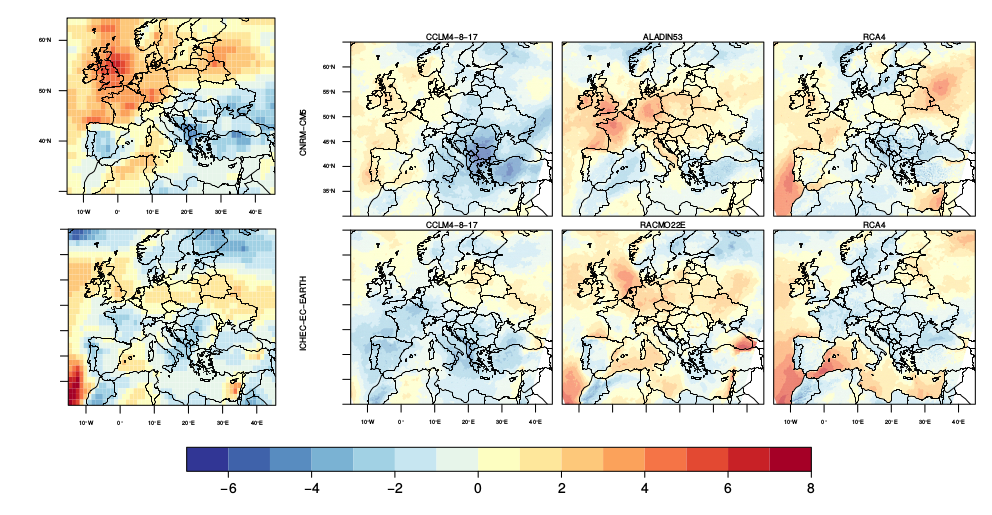
\includegraphics[scale=0.3]{clt_gimp3.png}
        \centering\caption{CLT change (1971/2000)-(2021/2050) ($\%$)}
      \end{figure}
\end{frame}
 
\begin{frame}[fragile]{CLT mean changes 2021-2050}
\vspace{1\baselineskip}
\begin{columns}
  \begin{column}{0.7\textwidth}
    \hspace{2\baselineskip}\LARGE{\textbf{GCM}}
%      \end{column}
%      \begin{column}{0.7\textwidth}
        \hspace{3.8\baselineskip}{\LARGE{\textbf{RCM}}}
%   \end{column}
%   \end{columns}
    \begin{figure}
      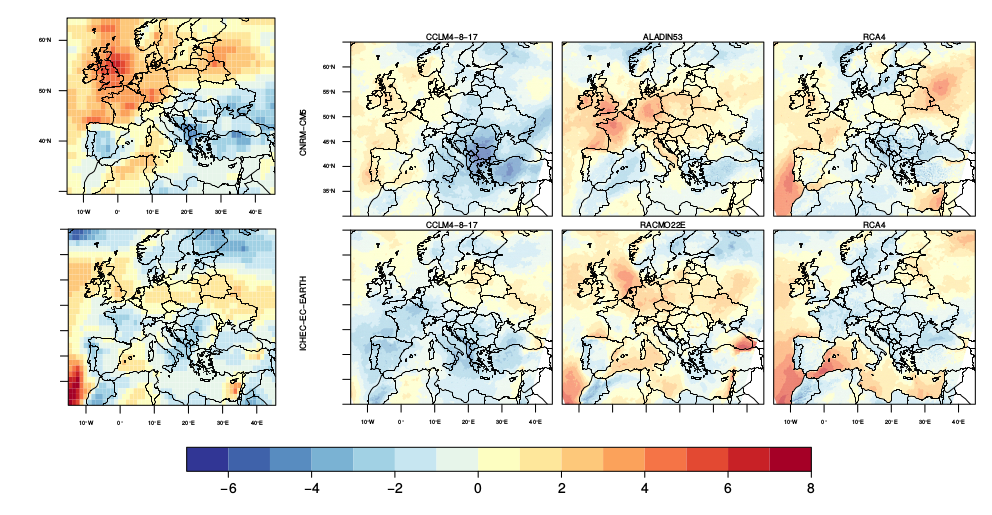
\includegraphics[scale=0.26]{clt_gimp3.png}
        \centering\caption{CLT change (1971/2000)-(2021/2050) ($\%$)}
    \end{figure}
  \end{column}
  \begin{column}{0.4\textwidth}
      \begin{itemize}
        \centering\vspace{0.05\baselineskip}\item RCMs without evolving aerosols: CLT spatial pattern can explain SSR spatial pattern.
        \centering\item CLT spatial pattern cannot explain SSR spatial pattern in models with evolving aerosols.
      \end{itemize}
    \end{column}
    \end{columns}
\end{frame}

% \begin{frame}[fragile]{CLT mean changes 2021-2050}
% %\vspace{1\baselineskip}
% \begin{columns}
%   \begin{column}{0.45\textwidth}
%     \centering{\hspace{4\baslineskip}\LARGE{\textbf{GCM}}}
%       \end{column}
%       \begin{column}{0.7\textwidth}
%         \hspace{5.2\baselineskip}{\LARGE{\textbf{RCM}}}
%    \end{column}
%    \end{columns}
%     \begin{figure}
%       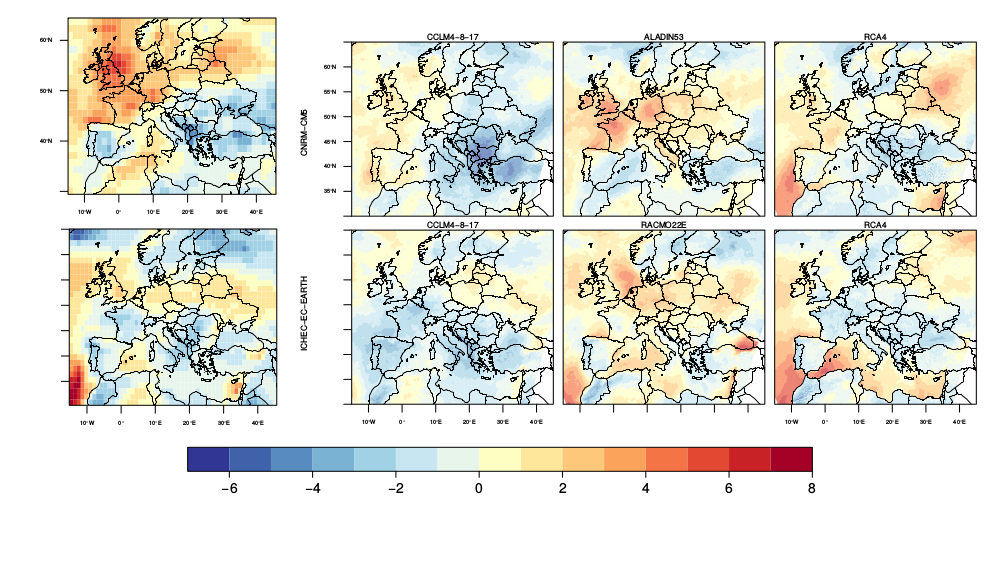
\includegraphics[scale=0.3]{clt_gimp2.png}
%         \centering\caption{CLT change (1971/2000)-(2021/2050) ($\%$)}
%       \end{figure}
%     \vspace{0.01\baselineskip}
%       \begin{itemize}
%       \item No clear relationship between SSR and CLT.
%       \end{itemize}
% \end{frame}


\begin{frame}[fragile]{Mean changes 2021-2050}
  \begin{table}
    {\small{
    \centering{\begin{tabular}[1\textwidth]{c|c|c|c}
      \toprule
      GCM & RCM & $\Delta{SSR}$ [$W/m^2$] & $\Delta{CLT}$ [$\%$]\\
                 \midrule
                 CNRM-CM5 &  & \textbf{9.9} & 0.5\\
                & CCLM4-8-17 & -2.4& -0.8 \\
                & \alert{ALADIN53} & \textbf{12.6}& 0.3\\
                & RCA4 & -2.6 & 0.2 \\
                 \midrule
                 EC-EARTH & & \textbf{5.6}& -0.3\\
                & CCLM4-8-17 & -2.7 & -0.9\\
                & \alert{RACMO22E} & \textbf{4.8}& 0.5\\
                & RCA4 & -2.1 & 0.1\\
      \bottomrule
               \end{tabular}}
             \vspace{0.75\baselineskip}
             \caption{Spatial changes in SSR and CLT}
     \end{table}}}
\end{frame}

\begin{frame}[fragile]{AOD mean changes 2021-2050}
  \begin{columns}
   \begin{column}{0.5\textwidth}
      \begin{figure}
         \centering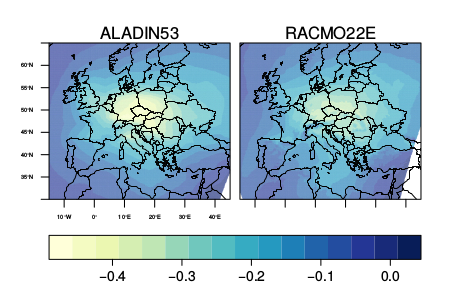
\includegraphics[scale=0.5]{aod.png}
     \centering\caption{AOD change (1971/2000)-(2021/2050)}
   \end{figure}
     \end{column}
     \begin{column}{0.6\textwidth}
       \begin{itemize}
       \item Spatial pattern of $\Delta{AOD}$ similar to $\Delta{SSR}$ when evolving aerosols considered.
       \item Higher correltation of SSR with AOD than with CLT.
       \end{itemize}
     \end{column}
   \end{columns}   
  \begin{table}
    {\tiny{
    \centering{\begin{tabular}[1\textwidth]{c|c|c|c|c}
      \toprule
      GCM & RCM & $\Delta{AOD}$ & $\rho_{SSR,CLT}$ & $\rho_{SSR,AOD}$\\
                 \midrule
                & CCLM4-8-17 & - & -0.7 & -\\
                CNRM-CM5& \alert{ALADIN53} & -0.2 & -0.2& -0.9 \\
                & RCA4 & - & -0.8& -\\
                 \midrule 
                & CCLM4-8-17 & - & -0.8 & - \\
                EC-EARTH& \alert{RACMO22E} & -0.1 & -0.3 & -0.6\\
                & RCA4 & - & -0.8 & -\\
      \bottomrule
               \end{tabular}}
           \end{table}}}
\end{frame}
 

\subsection{$\Delta{PV}$ by country}
 
\begin{frame}[fragile]{$\Delta$PV relative JJA mean by country}
     \begin{figure}
       \centering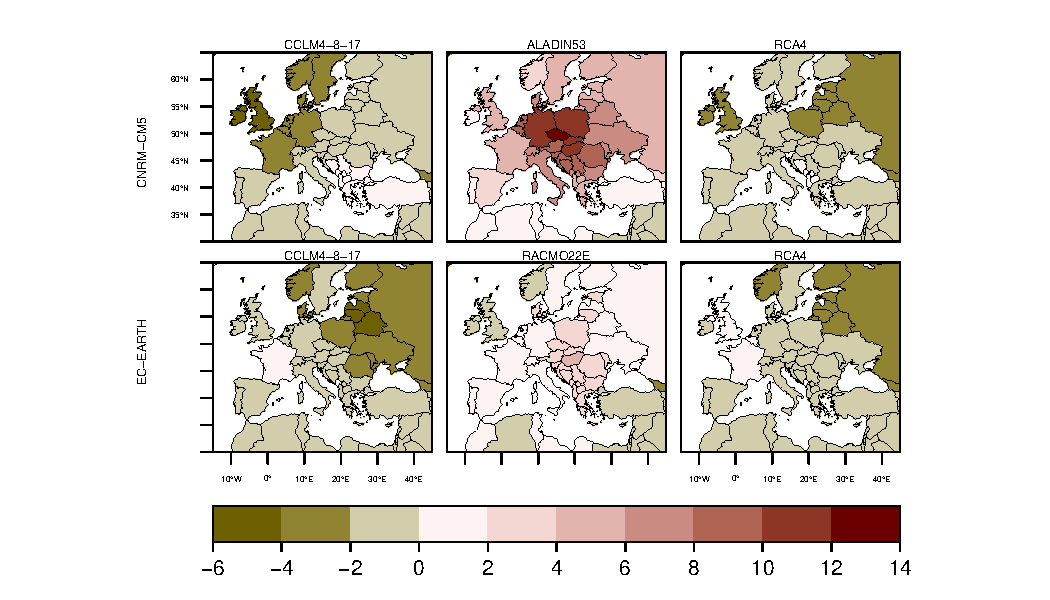
\includegraphics[scale=0.65]{bycountryJJArelative_area_newscriptall5}
       \caption{Relative change in PV potential [\%]}
     \end{figure}
\end{frame}

% \begin{frame}[fragile]{$\Delta$PV relative JJA mean by country}
%   \vspace{0.5\baselineskip}
%      \begin{figure}
%        \centering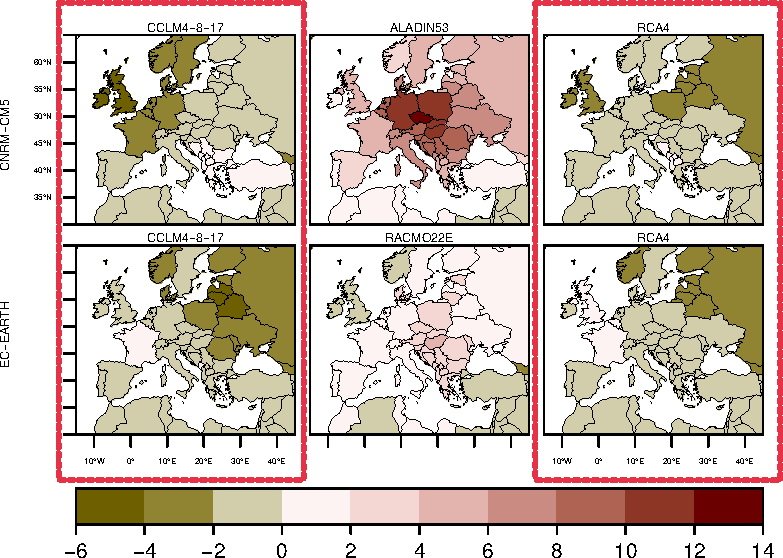
\includegraphics[scale=0.5]{bycountryJJArelative_area_newscriptall5_2}
%        \centering\caption{Relative change in PV potential [\%]}
%      \end{figure}
%      \begin{itemize}
%      \item Decrease for models with no-evolving aerosols  
%        \end{itemize}
% \end{frame}

\begin{frame}[fragile]{$\Delta$PV relative JJA mean by country}
  \vspace{0.5\baselineskip}
  \begin{columns}
    \begin{column}{0.6\textwidth}
  \begin{figure}
       \centering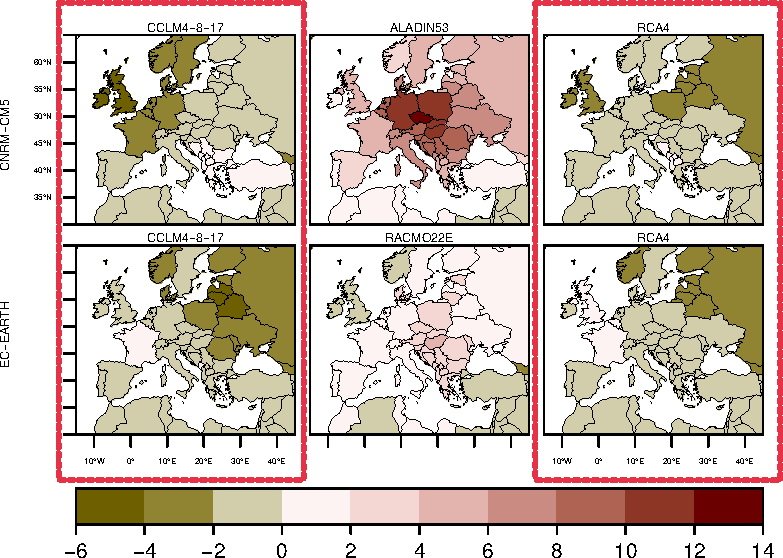
\includegraphics[scale=0.5]{bycountryJJArelative_area_newscriptall5_2}
       \centering\caption{Relative change in PV potential [\%]}
     \end{figure}
   \end{column}
   \begin{column}{0.4\textwidth}
     \begin{itemize}
     \item Decrease for models with no-evolving aerosols.
     \end{itemize}
     \end{column}
     \end{columns}
\end{frame}

\begin{frame}[fragile]{$\Delta$PV relative JJA mean by country}
  \vspace{0.5\baselineskip}
  \begin{columns}
    \begin{column}{0.6\textwidth}
  \begin{figure}
       \centering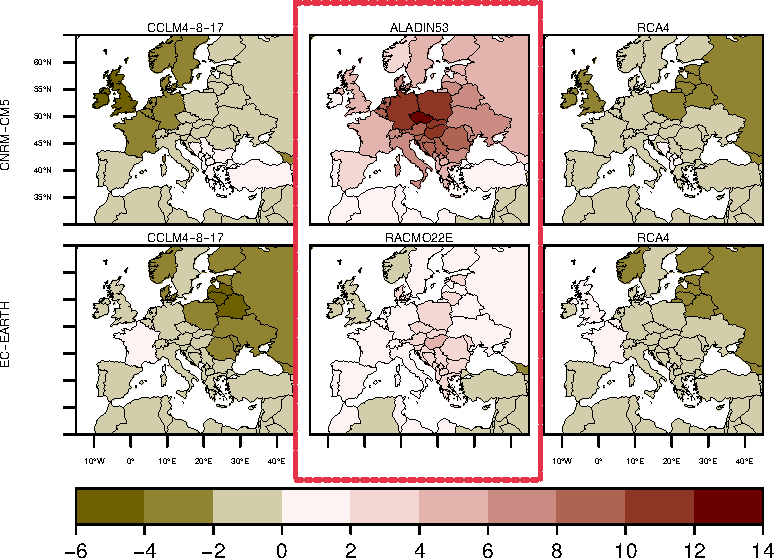
\includegraphics[scale=0.5]{bycountryJJArelative_area_newscriptall5_3}
       \centering\caption{Relative change in PV potential [\%]}
     \end{figure}
   \end{column}
   \begin{column}{0.4\textwidth}
     \begin{itemize}
     \item Decrease for models with no-evolving aerosols.
     \item Increase for models with evolving aerosols.
     \item Central-Europe is the most impacted area.  
     \end{itemize}
     \end{column}
     \end{columns}
\end{frame}

% \begin{frame}[fragile]{}
%   \begin{figure}
%     {\alert{Anomalía de radiación (JJA) 2050/2021-2000/1971}}
%         \centering\includegraphics[scale=0.55]{diferences_ssr_newperiods_9abr.pdf}\\
%         %\centering\includegraphics[scale=0.45]{diferences_clt_newperiods_9abr.pdf}
%         \tiny{\centering\caption{Anomal\'ia de radiaci\'on en superficie (2021/2050)-(1971/2000) ($W/m^2$)}}
%       \end{figure}
%       \begin{itemize}
%       \item <1->Diferentes patrones espaciales en la anomal\'ia
%       \item <1->CNRM-ALADIN5.3 presenta incremento generalizado
%       \end{itemize}
% \end{frame}

% \begin{frame}[plain]{RCP4.5}
%   \begin{figure}
%     {\alert{Anomalía de nubosidad (JJA) 2050/2021-2000/1971}}
%       \centering\includegraphics[scale=0.55]{diferences_clt_newperiods_9abr.pdf}
%      \centering\caption{Anomal\'ia de la cubierta nubosa  (2021/2050)-(1971/2000) for ALADIN5.3 ($\%$)}
%    \end{figure}
%    \begin{itemize}
%    \item Descenso de la nubosidad.
%    \item Correlaci\'on espacial entre SSR y CLT mayor para ENEA-PROTHEUS (-0.6 vs -0.9).  
%    \end{itemize}
% \end{frame}

% \begin{frame}[fragile]{RCP4.5}
% Anomal\'ias para todo el dominio de ambas variables:  
%  \begin{table}
%     \caption{Simulaciones de RCM utilizadas}
%     \begin{tabular}{c|c|c}
%       \toprule
%       Modelo & SSR [$W/m^2$] & CLT [$\%$] \\
%       \midrule
%       ENEA-PROTHEUS & 0.67 & -1.76 \\
%       CNRM-ALADIN5.3 & 6.83 & -1.17\\
%       \bottomrule
%     \end{tabular}
%   \end{table}  
% \end{frame}

\section{Conclusions}

\begin{frame}[fragile]{Conclusions}
\begin{alertblock}{}
    \begin{itemize}
    \item  For the mid century, an \textbf{\alert{increase}} in \textbf{photovoltaic potential} is projected over Europe when the \textbf{evolution} of \textbf{aerosols} over the area is considered.
    \item The \textbf{magnitude} depends on the country and the models.
    \item The most impacted areas are in Central-Europe, with an important potential increase of more than \textbf{10\%} but large uncertainty between models.
    \end{itemize}
\end{alertblock}
\begin{alertblock}{Perspectives}
\begin{itemize}
\item A \textbf{robust answer} is needed in order to deliver key messages for the solar industry.
\item The FPS-aerosols could help to understand uncertainties and develop better projections for energy purposes.  
% \item  La representación de los aerosoles en las \textbf{proyecciones de CC.} influyen en las variables relevantes para el potencial fotovoltaico.
\end{itemize}
\end{alertblock}
\end{frame}

% \begin{frame}{Perspectivas}
% \begin{alertblock}{Análisis multimodelo EURO-CORDEX}
% Estudio de la influencia de los aerosoles en escenarios de CC. sobre la radiación y la producción fotovoltaica con un 'ensemble' de modelos.
% \end{alertblock}
% \begin{alertblock}{}
%   \begin{itemize}
% \item Resultados robustos sobre la \textbf{evoluci\'on} del recurso solar. 
% \item Importancia en el desarrollo de los \textbf{servicios clim\'aticos}.
% \end{itemize}
% \end{alertblock}
% \end{frame}

\begin{frame}[standout]
    Thank you for your attention.\\ 
\vspace{2\baselineskip}\small{claudia.gutierrez@uclm.es}
\end{frame}

\end{document}


            
